%!TEX program=xelatex

\documentclass[12pt]{article}
\usepackage{example}
%% Отрисовка границ полей (для отладки)
% \usepackage{showframe}

%% Для возможности вставки ссылок (\url)
\usepackage{hyperref}

\usepackage{subcaption}
\usepackage{amsmath}
\usepackage{caption}
\usepackage{subcaption}
\usepackage{graphicx}
\usepackage{pdflscape}

\usepackage[utf8]{inputenc}


% \usepackage[parentracker=true,
% backend=biber,
% hyperref=false,
% style=gost-numeric,
% language=auto,
% autolang=other,
% citestyle=gost-numeric,
% defernumbers=true,
% bibstyle=gost-numeric,
% sorting=ntvy,
% ]{biblatex}
% \addbibresource{refs.bib}

%% Определение переменных
\affiliation{Кафедра математической физики}
\author{Певцов Артём Алексеевич}
\title{Гибридный метод нежёсткого совмещения изображений клеточных структур}
\worktype{ВЫПУСКНАЯ КВАЛИФИКАЦИОННАЯ РАБОТА}
\supervisor{к.ф-м.н., c.н.с.\\Д.В.Сорокин}
\date{Москва, \the\year{}}

\newfontfamily{\cyrillicfonttt}{Courier New}

\begin{document}

% \bibliographystyle{unsrt} \bibliography{refs}
\maketitle
\maketoc

%% Тут начинается основной текст

\section{Введение}

Анализ движения клеток и субклеточных структур в последовательностях микроскопических изображений (Рис. 1) очень
важен в задачах клеточной биологии. Он используется для лучшего понимания биологических процессов, таких как репликация ДНК, репарация ДНК, защита от вирусов\cite{Leonard2019dnarep} \cite{Sotiras2013deformable}. Движение клетки
представляет собой совокупность ее локального и глобального движений. Для компенсации глобального движения и деформации последовательностей живых клеток в биомедицинском анализе
применяются различные методы совмещения изображений. Поскольку клетка не только движется, но
и меняет свою форму с течением времени, компенсация такого движения - это очень сложная задача.
С помощью методов совмещения все изображения последовательности выравниваются по опорному
кадру, которым обычно является первое изображением последовательности.
Таким образом, совмещение изображений помогает определить и проанализировать
локальное движение субклеточных частиц, которое обычно наиболее важно для исследований.
\begin{figure}[h]
    \centering
    \subfloat[]{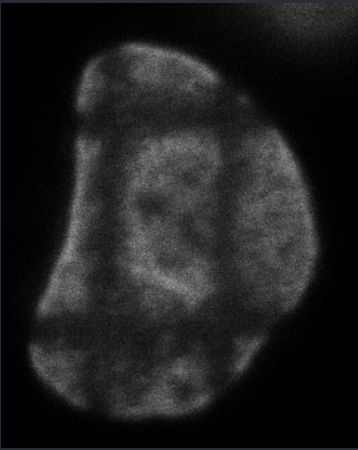
\includegraphics[width=3in,height=3.5in]{cell}}\quad
    \subfloat[]{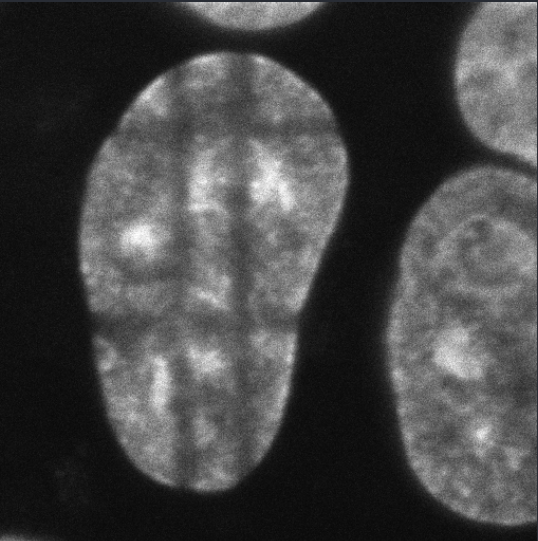
\includegraphics[width=3in,height=3.5in]{cell_2}}
    \caption{Примеры входных изображений}
    \label{fig1}
\end{figure}

Предыдущие работы по методам совмещения биомедицинских изображений можно разделить на две группы: классические подходы и подходы, основанные на обучении. 
Среди классических методов существуют
подходы, основанные на интенсивности: в работах \cite{goobic2005}  и \cite{wilson2006} 
авторы использовали информацию о корреляции интенсивностей, для жесткого совмещения. В работе \cite{vandegiessen2011} описывается
метод, который оценивает затухание, моделируя фотообесцвечивание в виде экспоненциально затухающих сигналов. 
В работе \cite{raza2012}  авторы предложили метод блочного совмещения на цветных изображениях флуоресцентной микроскопии.
В работе \cite{ozere2013}  был представлен метод параметрической стабилизации для оценки глобального движения и изменения интенсивности.
Другие классические методы не учитывают интенсивность:
существует подход, основанный на контурах, который выполняет нежесткое совмещение \cite{sorokin2018} ; авторы использовали динамическую модель упругости для прямого моделирования движения ядра и
смещения на основе движения его контуров. В \cite{matula2006} , авторы предложили использовать информацию о расположении субклеточных структур для получения жесткого преобразования между последовательными
изображениями. Кроме того, существуют методы, опирающиеся на оптический поток, который основан
на моделях движения клеток или других физических принципах и доказал свою эффективность в практическом применении.
В работе \cite{kim2010}  авторы использовали модель оптического потока Лукаса-Канаде для оценки поля смещения между последовательными кадрами. 
Затем эта работа была продолжена \cite{tektonidis2015}, где авторы добавили
многокадровое расширение и повышенную помехоустойчивость. 


Методы, основанные на обучении чаще всего базируются на использовании нейронных сетей. Так, например, в \cite{anoshina2024} архитектура сверточной
нейронной сети состоит из двух частей: сети локализации для оценки аффинного преобразования и U-Net-подобной сети для оценки поля смещения. В статье \cite{boveiri2024} сравниваются все современные нейросетевые подходы к совмещению биомедицинских изображений. Как итог (в данной статье) один из лучших результатов показывают пространственные сети трансформеры. В последнее время для решения задачи совмещения всё чаще используются методы, основанные на нейронных операторах \cite{drozdovresolution}. 


Рассматриваемый в данной работе контурный метод совмещения изображений опирается на решение уравнения Навье, описывающее смещение упругой среды. Традиционно его решают численными методами, что при высоких разрешениях и сложной геометрии оказывается вычислительно затратным. В последние годы для аппроксимации подобных дифференциальных операторов активно применяются нейронные операторы, способные обучаться напрямую на решениях уравнений и затем предсказывать их при различных граничных условиях. Рассмотрим некоторые из них.

 
Модель Fourier Neural Operator (FNO) впервые была представлена как метод для обучения операторов между бесконечномерными функциями с помощью параметризации ядра интегрального оператора в спектральном пространстве посредством быстрого преобразования Фурье \cite{fno1}. 

FNO доказала высокую эффективность при решении задач Бюргерса, Дэрси и уравнений Навье–Стокса. Модель обучается на одной дискретизации задачи, а затем обрабатывает данные на произвольной сетке более высокой  плотности без изменения весов и без потери качества, а также даёт ускорение до трёх порядков, по сравнению с традиционными численными методами\cite{fno1}. При этом FNO обладает универсальной способностью аппроксимации непрерывных операторов и инвариантностью к дискретизации, что подтверждается теоретическими результатами\cite{fno2}.


Для повышения качества аппроксимации классической архитектуры FNO в задачах моделирования многофазных потоков предложена модификация  U-net based Fourier Neural Operator (U-FNO). В неё интегрирован U-подобный путь аналогично U-Net, который последовательно обрабатывает спектральные представления и позволяет эффективнее захватывать локальные и глобальные зависимости \cite{ufno1}. Экспериментальная оценка на задачах прогнозирования газонасыщенности и развития давления в CO$_2$–водной мультифазной среде показала, что U-FNO достигает более высокой точности по сравнению с базовой CNN-архитектурой, при этом требуя лишь около трети объёма обучающих данных и демонстрируя заметное ускорение вычислений и повышенную устойчивость к изменению геологических условий \cite{ufno1}.

Модель U-shaped Neural Operator (U-NO) реализует универсальный операторный подход в виде архитектуры, подобной сети U-net: входная функция сначала обрабатывается локальными сверточными блоками, затем проходит через спектральные слои для захвата глобальных зависимостей, и, наконец, в декодере через симметричные свёртки восстанавливает исходную размерность представления \cite{uno1}. Такой U-путь обеспечивает эффективное комбинирование локальных и глобальных признаков, что повышает способность модели аппроксимировать несжимаемые операторы и сохранять инвариантность к изменению сетки. В сравнительных экспериментах U-NO продемонстрировала более высокую точность и устойчивость при решении нелинейных дифференциальных уравнений по сравнению с классическими FNO и CNN-архитектурами, одновременно снижая потребность в обучающих данных и вычислительных ресурсах \cite{uno1}.

Для решения задач, в которых оператор зависит от нескольких входных функций, предложена архитектура Multiple-Input Operator Network (MIONet). Основная идея заключается в том, что каждая входная функция кодируется своей входной веткой, после чего полученные представления объединяются и обрабатываются основной сетью, отвечающей за аппроксимацию выходного оператора на пространственном домене \cite{mionet1}. Впоследствии эта модель была опубликована в SIAM Journal on Scientific Computing с детальным обоснованием универсальной теоремы аппроксимации множественных входных операторов и анализом погрешностей 
\cite{mionet1}. Экспериментальные результаты продемонстрировали, что MIONet эффективно обучается на примерах систем ОДУ с разнообразными типами входных данных (начальные и граничные условия, внешние источники), существенно расширяя возможности применения нейронных операторов и повышая точность прогноза сложных физических процессов.



В данной работе рассматривается подход основанный на обработке двумерных контуров для компенсации глобального движения клеточного ядра.
Данный метод компенсации состоит из двух основных этапов. На первом этапе применяется 
жесткое совмещение для компенсации перемещения и вращения ядра. Это позволяет выровнять 
изображения относительно ядра клетки, устраняя глобальное движение.
На втором этапе - для более реалистичного моделирования смещения ядра решается уравнение Навье, для построения поля внутреннего смещения клетки при изменении её формы в процессе движения 
и последующей компенсации этого смещения.
Такой подход позволяет точно и эффективно компенсировать глобальное движение клеточного ядра при обработке последовательностей изображений реальных клеток.
В данной работе рассматривается несколько подходов к решению уравнения Навье - с помощью метода конечных элементов, классических нейронных операторов и нейронных операторов, использующих информацию об интенсивности.
Первый подход не использует информацию об интенсивности изображения, а сразу принимает на вход бинарную маску ядра.
Подход, основанный только на информации о контурах оказывается
особенно полезен, так как у входных изображений средняя интенсивность может сильно варьироваться.
Сначала устанавливаются соответствия между точками контуров
клетки на двух последовательных изображениях с использованием
алгоритма жёсткого совмещения, определяющего смещения границ
клетки. Затем строится поле смещений точек ядра, соответствующее его дефрмации, путем интерполяции смещений граничных точек ядра
с использованием метода конечных элементов. Данный подход был успешно применен к последовательностям изображений, полученных с помощью микроскопии реальных живых клеток.
В результате на данном этапе удалось получить сравнимые результаты с \cite{sorokin2014nonrigid}, но с использованием более современных методов программирования, что 
расширяет спектр возможностей дальнейшего исследования.

Благодаря реализованному на первом этапе алгоритму удалось генерировать данные для обучения нейронных операторов, таких как FNO и U-NO. Подход с использованием U-NO показал качество лучшее, чем основанный на  МКЭ. Для улучшения качества работы модели было решено дополнительно при обучении моделей подавать на вход информацию об интенсивности изображений, которая учитывалась в функции потерь, что дало лучшее качество на нескольких последовательностях.





\section{Цель работы}

Целью работы является реализация метода совмещения изображений живых клеток на основе упругой модели, состоящего из нескольких этапов:

\begin{enumerate}
 \item Реализация метода жесткого совмещения границ клеток для последовательности изображений
 \item Разработка метода решения уравнения Навье с помощью МКЭ для нежесткого совмещения клеток на последовательности изображений
 \item Разработка нейросетевого метода решения уравнения Навье для нежесткого совмещения клеток на последовательности изображений
 \item Анализ полученных результатов.
\end{enumerate}

\section{Постановка задачи}

Задача совмещения последовательности изображений ставится следующим образом. На вход системы подаётся упорядоченная последовательность биомедицинских изображений вместе с соответствующими масками
\[
\{(I_k, S_k)\}_{k=0}^N,
\]
где
\begin{itemize}
  \item $I_0$ — опорное (fixed) изображение, к которому необходимо привести все остальные,
  \item $I_k$ — движущееся (moving) изображение на $k$–м шаге,
  \item $S_k$ — маска, соответствующая изображению $I_k$.
\end{itemize}

Требуется найти семейство преобразований
\[
\{u_k\colon \mathbb{R}^2 \to \mathbb{R}^2\}_{k=1}^N
\]
таких, что каждую пару $(I_{k}, S_k)$ можно совместить, а итоговое смещение всех изображений к $I_0$ задаётся композицией
\[
U_{0\leftarrow N} \;=\; u_1 \circ u_2 \circ \cdots \circ u_N.
\]

Задача сводится к последовательному решению $k$ задач парного совмещения:
\[
\hat u_k \;=\;\arg\min_{u}\; \mathcal{L}\bigl(I_{k-1},\ I_{k},\, S_k,\, S_{k-1},\ u\bigr),
\quad k = 1,2,\dots,N,
\]
где
\begin{itemize}
  \item $u$ — поле смещения, применяемое к moving image;
  \item $\mathcal{L}$ — функционал потерь;
  \item $I_{k-1}$, $M_{k}$ — изображение и маска на шаге $k-1$ (fixed image);
  \item $S_{k}$, $M_k$ — изображение и маска на шаге $k$ (moving image) ;
\end{itemize}

Для повышения качества и устойчивости совмещения изображений, обычно сначала выполняют жёсткое (аффинное) совмещение:
\[
M_k^{\mathrm{aff}}\;=\;\arg\min_{u\,\in\,\mathrm{Aff}}\;
\mathcal{L}_{\mathrm{aff}}\bigl(I_{k-1},\, I_{k}, M_{k-1}, M_{k},\, u\bigr),
\]
где $\mathrm{Aff}$ — пространство аффинных преобразований. После этого решается задача нежёсткого совмещения с помощью уравнения Навье.

Требуется разработать гибридный метод нежёсткого совмещения биомедицинских изображений, протестировать его на четырех последовательностях изображений ядер живых клеток и сравнить с другими методами совмещения.



\section{Реализация метода жесткого совмещения границ клеток для последовательности изображений}

\subsection{Алгоритм дискретизации границ клеток}

Работа алгоритма начинается с выделения дискретного контура $c(p) = [x_p, y_p]$ из бинаризированного изображения клетки, полученного заранее при помощи методов
пороговой сегментации.  

Для выделения контура шириной в один пиксель из маски вычитается результат применения морфологической эрозии с ядром $$I = \begin{bmatrix}
    0 & 1 & 0 \\
    1 & 1 & 1 \\
    0 & 1 & 0 \\
    \end{bmatrix}$$ к этой маске.
После чего полученные точки контура упорядочиваются, используя цепные методы.\cite{annapurna2013} 

Как итог мы получаем
последовательность пар чисел с координатами точек границ для каждого изображения из стопки, которые в дальнейшем будем использовать как для жёсткого
совмещения границ, так и для определения граничных условий уравнения Навье.


\subsection{Метод жёсткого совмещения границ для последовательности изображений}
В нашем подходе к совмещению используется стратегия последовательного выравнивания при которой
для каждого изображение стопки последовательно подбираются преобразования, переводящие данный контур к базовому (чаще всего первому).
Выравнивание выполняется следующим образом. На каждом шаге алгоритма мы будем находить матрицу преобразования k-ого контура к контуру k+1-ого  изображения.
Сначала мы находим линейные преобразования $M_k^{k+1}(\theta, t)$
от кадра k + 1 до кадра k (k =
1, . . . , N − 1, $\theta$ - угол поворота, а t - вектор перемещения).
Затем, чтобы определить преобразование $M_1^{k}(\theta, t)$ из кадра k в первый
кадр, мы перемножаем матрицы преобразования:
$$M_1^{k}(\theta, t) = M_{k}^{k-1}(\theta, t) M_1^{k-1}(\theta, t) \quad k\geq2 $$


Когда все преобразования $M_{k}^{k-1}(\theta, t)$ построены, они применяются к соответствующим изображениям
последовательности. 

Для описания каждого контура создается одномерная функция, называемая контурным дескриптором \cite{devylder2011}. Мы используем
дескриптор основывающийся на расстоянии до центра клетки:

$$ s(p) = \frac{\|c(p) - r_{\text{cm}}\|}{\sum_{i=1}^{N} \|c(p_i) - r_{\text{cm}}\|} $$ 
Где $r_{cm}$ - это центроид ядра. Поскольку дескрипторы являются
периодическими с периодом M, мы можем ограничить наш анализ только одним
периодом (p = 1, ... , M) без потери общности.


Чтобы найти преобразование $M_{k}^{k-1}(\theta, t)$, сначала устанавливается взаимно однозначное соответствие между точками границ клеток
в кадрах k и k + 1. Мы используем взаимную корреляцию между дескрипторами контуров, чтобы найти оптимальный сдвиг $\tau$ между их начальными точками:

$$ \tau = \text{argmax}_{\mu} \left( \rho(s_k, s_{k+1}) \right)$$

Где $\rho$ - это функция корреляции. Затем второй контур циклически сдвигается на полученное значение $\tau$, чтобы установить правильную нумерацию точек контура.
После того, как соответствие установлено вычисляются аналитически параметры преобразования θ и t\cite{annapurna2013}. Для этого нужно минимизировать функцию

$$\sum_{i=0}^{n} || c_k(p) - R(\theta) c'_{k+1}(p) - t||$$

Где $c'_{k+1}(p)$ - циклически сдвинутый на $\tau$ контур, а $R(\theta)$ - матрица поворота. Минимизируется же данная функция 
с помощью метода наименьших квадратов.



\section{Метод решения уравнения Навье с помощью МКЭ}
Как показывают исследования клеточное ядро ведёт себя эластично\cite{tseng2004}, а значит смещение ядра можно смоделировать 
с помощью линейной теории упругости, а именно с помощью уравнения Навье 
с граничными условиями типа Дирихле:

\begin{align*}
    \mu \Delta u(x) + (\mu + \lambda) \nabla(\nabla u(x)) &= 0, && x \in \Omega, \\
    u(x) &= u_0, && x \in \partial\Omega,
\end{align*}
где $\Omega$ - область, определяемая сегментацией клеточного ядра, $\partial\Omega$ - граница области, $u(x)$ обозначает смещение $u$ в точке $x$, $\nabla$ - оператор Набла, $\Delta$ - оператор Лапласа, а $\mu$ и $\lambda$ - коэффициенты Ламе.

Для построения поля смещения $u_{k}^{k-1}(x)$ задающего отображение
внутреннюю часть ядра в кадре k + 1 на внутреннюю часть ядра в кадре k нам нужно решить заданное уравнение.
Данное уравнение решается при помощи метода конечных элементов.
Для этого на каждом шагу граница второго изображения заново разбивалась на точки (Рис. 2) для улучшения соответствия двух контуров.
Каждая точка нового разбиения выбиралась как самая близкая точка к соответствующей точке первой границы.

Граничные условия Дирихле таким образом получаются как:

$$ u_0(c_k) = \widetilde{c}_{k-1}(p) - c_k(p)$$

где $\widetilde{c}_{k-1}(p)$ представляет точки границы ядра в
кадре k − 1, которые соответствуют точкам $c_k(p)$ кадра k.


\begin{figure}[h]
    \centering
    \subfloat[Контур до семплирования]{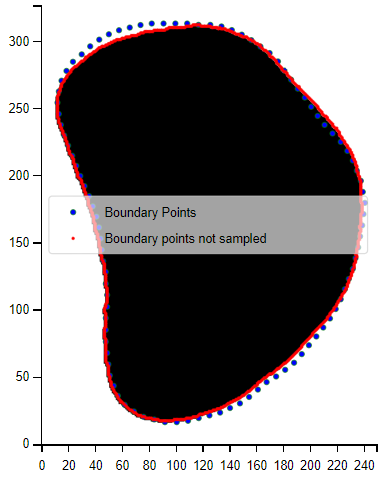
\includegraphics[width=3in,height=3.2in]{BP_ns.png}}\quad
    \subfloat[Контур после выбора нужных точек]{\includegraphics[width=3in,height=3in]{{BP_s.png}}}
    \caption{Семплирование контуров}
    \label{fig1}
\end{figure}

Далее внутренняя часть клетки триангулируется (Рис. 3) при помощи триангуляции Делоне\cite{weatherill1992} и 
итеративно рассчитывается внутреннее поле смещения при помощи метода конечных элементов\cite{alberty2002}.
Метод конечных элементов (МКЭ) - это численный метод, используемый для решения дифференциальных уравнений, таких как уравнение Навье, на границе тела с заданной триангуляцией. 
В основе МКЭ лежит аппроксимация решения дифференциального уравнения конечными функциями, называемыми конечными элементами.
Суть МКЭ заключается в том, чтобы объединить вычисления матриц жёсткости в каждом локальном элементе к общей аппроксимирующей матрице жёсткости всего тела.

Используя стандартный метод Галеркина, пространство \( H^1(X) \) аппроксимируется конечномерным подпространством \( S \). Задача сводится к нахождению \( u_h \in S \), такого что:
\begin{align}
\int_X \sigma(v_h) : C \sigma(u_h) \, dx = \int_X f \cdot v_h \, dx  \quad \forall v_h \in S,
\end{align}
где \( C \) — тензор упругих свойств материала.

\begin{figure}[h]
    \centering
    \subfloat[Пример триангуляции]{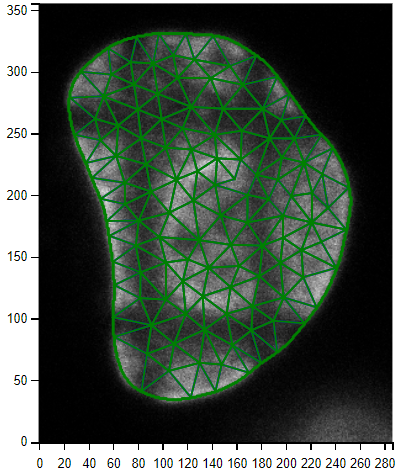
\includegraphics[width=3in,height=3.5in]{triang.png}}\quad
    \subfloat[Пример сопоставление контуров]{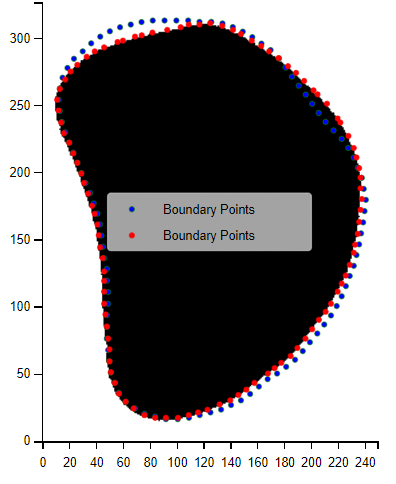
\includegraphics[width=3in,height=3.5in]{cont1.png}}
    \caption{Триангуляция и сопоставление контуров}
    \label{fig1}
\end{figure}

Конечный базисный вектор узлов задается как 

\( \{\mathbf{\mu}_1, \ldots, \mathbf{\mu}_{dN}\} = \{\phi_{1}e_1, \phi_{1}e_2, \ldots, \phi_{1}e_d, \ldots, \phi_{N}e_1, \phi_{N}e_2, \ldots, \phi_{N}e_d\} \), 
 где \( N \) - количество узлов сетки, \( d \) - размерность вектора смещения, и \( u_z \) - скалярная функция узла \( z \) в триангуляции \( T \),  \( \phi_z(z) = 1 \) и \( \phi_z(y) = 0 \) для всех \( y \in N \) с \( y \neq z \). Учитывая граничные условия.
 Перепишем (3) в терминах введённого базиса:

 \begin{align}
    \int_X \sigma(\mu_h) : C \sigma(u_h) \, dx = \int_X f \cdot \mu_k \, dx  \quad k = (1, \ldots, dN),
\end{align}


Представление данных о триангуляции включает в себя описание сетки узлов. Сетка задаётся файлами данных, которые описывают координаты каждой вершины.
Основная идея представления заключается в том, что данные об элементах и узлах сетки используются для построения матрицы жёсткости и вектора нагрузки:
\begin{align}
A_{jk} &= \sum_{T \in \mathcal{T}} \int_T \sigma(g_j) : C \sigma(g_k) \, dx, \\
b_j &= \sum_{T \in \mathcal{T}} \int_T f \cdot g_j \, dx,
\end{align}
где \( g_j \) и \( g_k \) — базисные функции, а \( \mathcal{T} \) и \( CN \) обозначают множества элементов сетки и граничных элементов соответственно.


Локальные матрицы жёсткости для каждого элемента сетки вычисляются на основе геометрических характеристик и материальных свойств. Для каждого треугольного элемента вычисления основаны на градиентах базисных функций:
\[
\text{STIMA}(T)_{kl} = \int_T \sigma(g_k) : C \sigma(g_l) \, dx,
\]
где \( \sigma(g) = \frac{1}{2}(\nabla g + (\nabla g)^T) \). После вычисления локальных матриц жёсткости, они ассемблируются в глобальную матрицу жёсткости, которая используется в дальнейших вычислениях для решения системы линейных уравнений.



\section{Нейросетевые методы решения уравнения Навье}

В последние годы методы глубокого обучения доказали свою эффективность для решения задач, связанных с уравнениями в частных производных (УЧП). Нейронные операторы сразу обучаются отображению между пространствами функций и позволяют предсказывать решения УЧП в любом новом положении параметров без многократного численного интегрирования.


\begin{figure}[h]
    \centering
    \subfloat[]{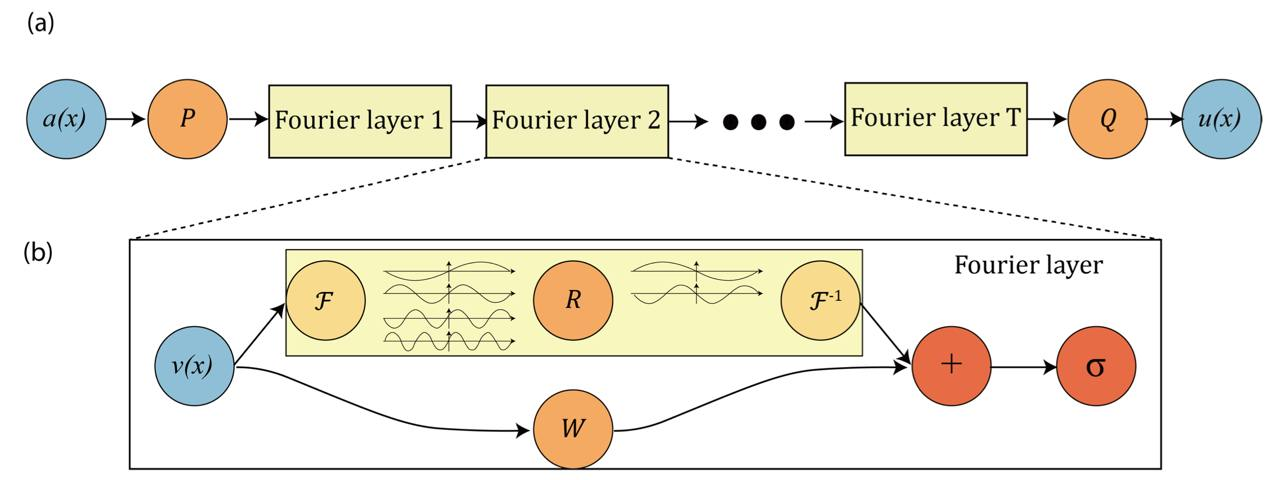
\includegraphics[width=6in,height=2.5in]{FNO2.jpg}}\quad

    \caption{Арихитектура FNO из \cite{li2021fourier} \
    (a) Полная архитектура нейронной сети \
    (b) FNO-слой}
    \label{fig1}
\end{figure}

\subsection{Метод FNO}  

Нейронный оператор Фурье обучает параметры спектральных слоёв для аппроксимации оператора решения УЧП \cite{fno1}.  
Архитектура включает (Рис. 4):
\begin{itemize}
  \item Слой трансляции, переводящий входные каналы в скрытое представление фиксированной размерности;
  \item Последовательность FNO-блоков: каждый блок состоит из спектральной свёртки (обработка первых $k$ гармоник в полученном представлении) и второго линейного слоя;
  \item Проекционный слой, возвращающий скрытое представление в пространство выходных каналов.
\end{itemize}
При подборе гиперпараметров исследовались:
\begin{itemize}
  \item диапазон количества мод в спектральных слоях;
  \item число скрытых каналов в каждом блоке;
  \item глубина сети (количество FNO-блоков);
  \item размер батча, число эпох и весовые коэффициенты регуляризации.
\end{itemize}
Обучение выполняется методом Adam с функцией потерь MSE для векторных полей смещения, проверка качества — на отложенной валидационной выборке, модели сохраняются по лучшей метрике.

\begin{figure}[h]
    \centering
    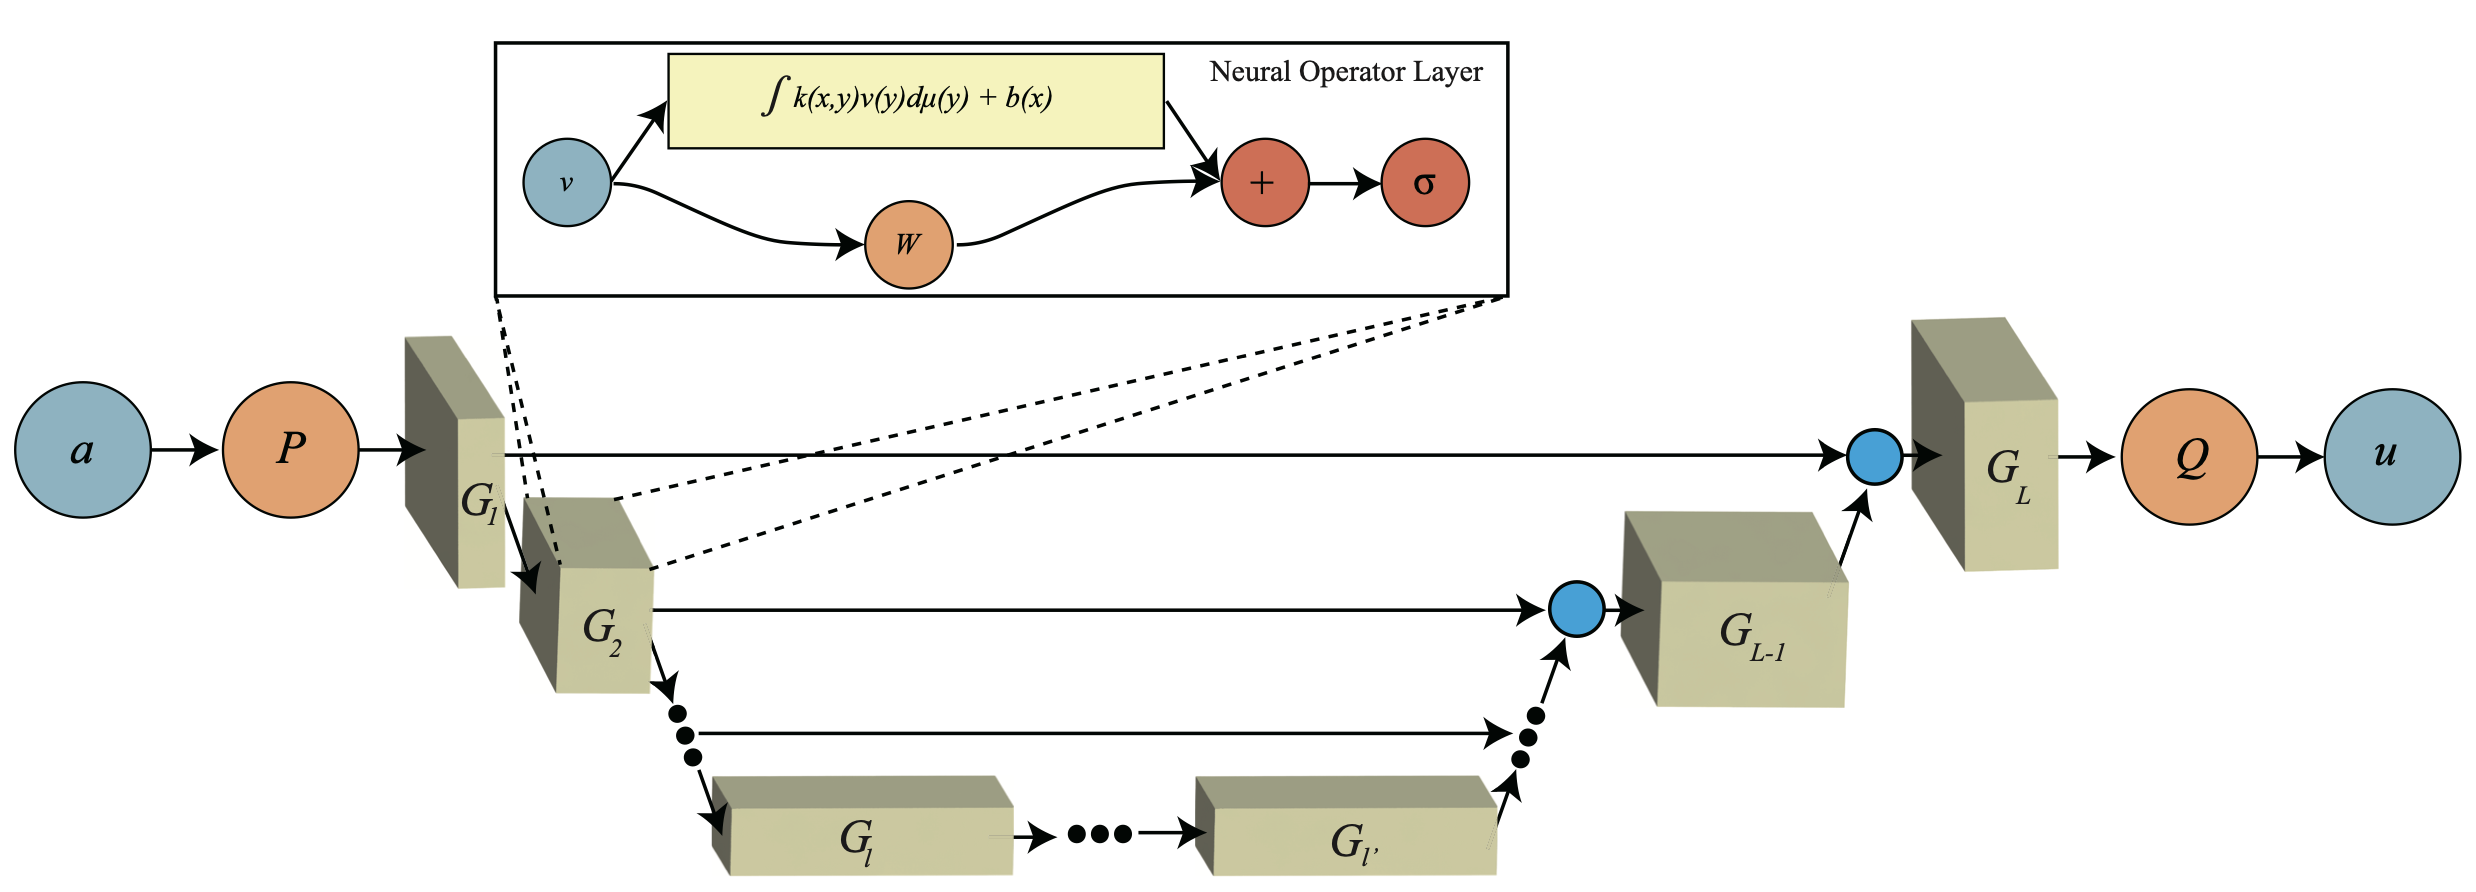
\includegraphics[width=6in,height=2.0in]{uno1.png}\quad

    \caption{Арихитектура U-NO из \cite{uno1}}
    \label{fig1}
\end{figure}


\subsection{Метод U-NO} 

U-shaped Neural Operator (U-NO) интегрирует U-образную структуру в спектральный подход \cite{uno1}.  
Основные компоненты (Рис. 5):
\begin{itemize}
  \item \emph{Encoder path}: чередование спектральных слоёв и понижающих преобразований для захвата глобальных контекстов;
  \item \emph{Decoder path}: обратные спектральные преобразования с поэтапным увеличением разрешения и пропуск слоёв, передающими высокочастотные признаки из encoder;
  \item нормализация и нелинейности между слоями для устойчивого обучения глубоких конфигураций.
\end{itemize}
При подборе гиперпараметров исследовались:
\begin{itemize}
  \item аналогичные параметры FNO
  \item глубина каждой ветви;
  \item параметры пропусков слоёв;
\end{itemize}


\subsection{Метод FNO с изменённой функцией потерь}  
Для повышения качества прогнозов на реальных микроскопических изображениях к стандартному MSE между полями смещения добавлено слагаемое, учитывающее отличия реконструированного интенсивностного кадра от второго реального кадра (Рис. 6):
\[
\mathcal{L} = \|\hat{\mathbf{u}} - \mathbf{u}\|_2^2 \;+\; \lambda_{\text{img}}\bigl\|\mathcal{W}(\mathbf{I}_1,\hat{\mathbf{u}})-\mathbf{I}_2\bigr\|_2^2.
\]
Оператор $\mathcal{W}$ (warping) реализован через дифференцируемую билинейную интерполяцию;
При подборе гиперпараметров исследовались:
\begin{itemize}
  \item аналогичные параметры FNO;
  \item $\lambda_{\text{img}}$  настраивается в ходе экспериментов;
  \item схема нормализации интенсивностей и выбор метода сглаживания потерь тоже подвергались перебору.
\end{itemize}
Такой подход стимулирует модель не только правильно предсказывать векторное поле, но и обеспечивать физически корректное преобразование интенсивностей.


\begin{figure}[h]
    \centering
    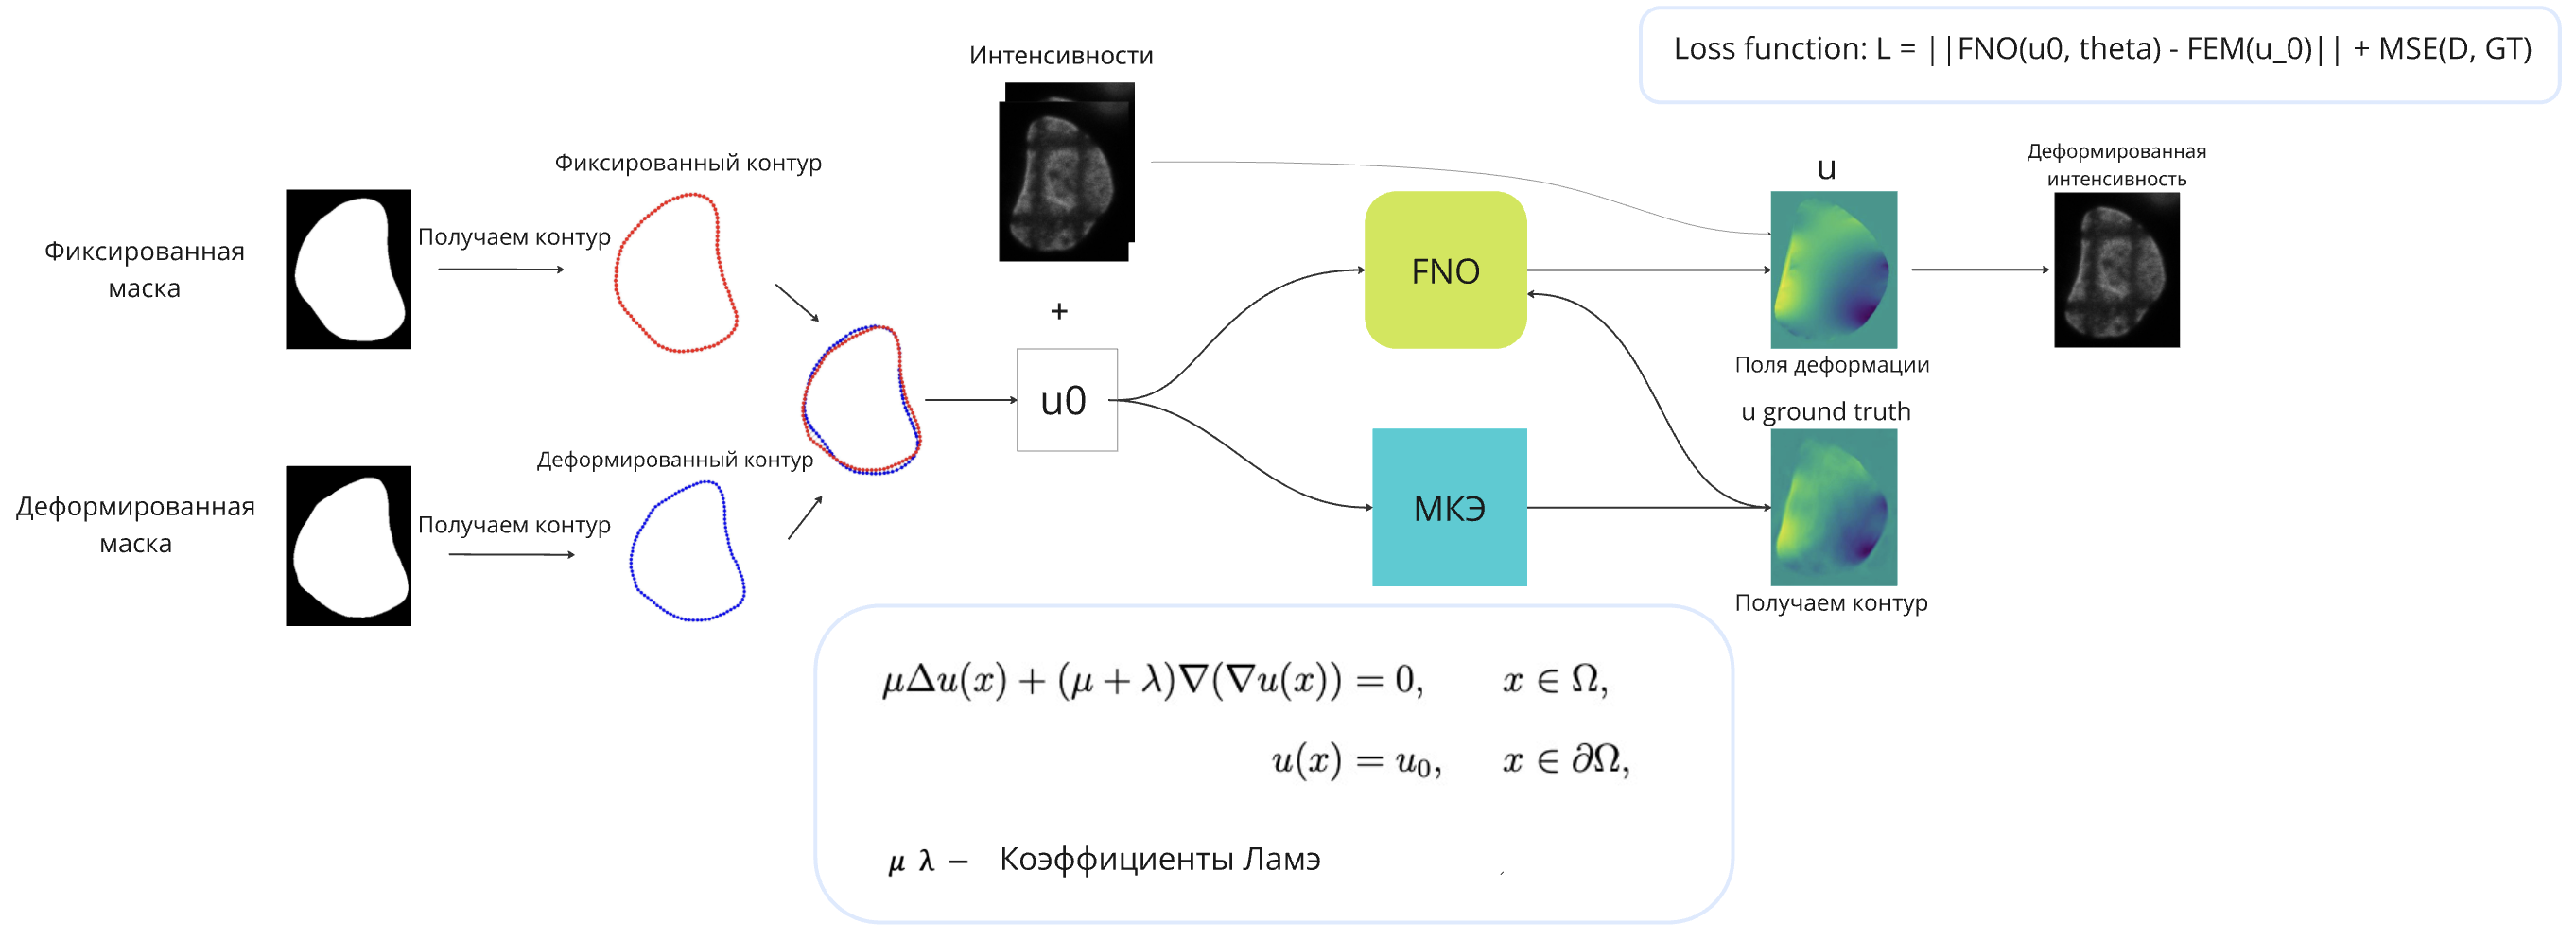
\includegraphics[width=1\linewidth]{fno_new_loss.png}

    \caption{Реализация подхода с изменённой функцией потерь}
    \label{fig1}
\end{figure}


\subsection{Обучение нейросетей}

Обучение всех трёх моделей (FNO, U-NO и FNO с модифицированной функцией потерь) велось по единому протоколу:

\begin{itemize}
  \item \textbf{Оптимизатор}: Adam \cite{kingma2014adam} с начальной скоростью обучения $\mathrm{lr}=0.001$, без учёта затухания весов (weight decay).
  \item \textbf{Функция потерь}: 
    \begin{itemize}
      \item для FNO и U-NO — стандартный MSE между предсказанным и истинным полями смещения;
      \item для FNO с новым loss — комбинированная функция
      \[
        \mathcal{L} = \|\hat{\mathbf{u}} - \mathbf{u}\|_2^2 \;+\; \lambda_{\text{img}}\bigl\|\mathcal{W}(\mathbf{I}_1,\hat{\mathbf{u}})-\mathbf{I}_2\bigr\|_2^2.
        \]
      где $\lambda_{\mathrm{disp}}$ подбираемый гиперпараметр.
    \end{itemize}
  \item \textbf{Загрузчики данных}:  
    пары изображений загружались через \verb|NPYDataset| и \verb|DataLoader|  
    входной и выходной тензоры переставлялись в формате \verb|[batch, channels, H, W]|. Размер батча составлял 32 пары.
    
  \item \textbf{Валидация}:  
    после каждой эпохи на отложенной выборке вычисляются средняя ошибка MSE и коэффициент детерминации $R^2$;  
    сохраняется модель с наилучшим значением валидационной ошибки.
\end{itemize}
\paragraph{Перебор гиперпараметров моделей}

Для каждой из рассматриваемых моделей был проведён систематический перебор ключевых гиперпараметров (Таблица 1) в следующих диапазонах:


\begin{itemize}
  \item \textbf{FNO}:
    \begin{itemize}
      \item число мод \verb|n_modes| $\in$ \{(16,16) (32,32), (64,64)\};
      \item количество скрытых каналов \verb|hidden_channels| $\in$ \{16, 32, 64\};
      \item число слоёв \verb|n_layers| $\in$ \{4, 6, 8\};
      \item число эпох обучения \verb|epochs| $\in$ \{120, 220, 320\}.
    \end{itemize}

  \item \textbf{FNO + новый функционал потерь}:
    \begin{itemize}
      \item \verb|n_modes| $\in$ \{(16,16), (32,32)\};
      \item \verb|hidden_channels| = 32;
      \item \verb|n_layers| $\in$ {6, 8};
      \item \verb|epochs| $\in$ \{120, 220, 320\};

      \item коэффициент в функции потерь перед ошибкой совмещения интенсивностей 
      
      
      $\lambda_{\text{disp}}$ $\in$ = \{0.001, 0.01, 0,1\}
          
    \end{itemize}

  \item \textbf{UNO}:
    \begin{itemize}
      \item число мод \verb|n_modes| $\in$ \{(16,16), (24,24)\};
      \item количество скрытых каналов \verb|hidden_channels| $\in$ \{32, 64\};
      \item число слоёв \verb|n_layers| $\in$ \{6, 8\};
      \item размеры выходных каналов каждого слоя \verb|uno_out_channels| $\in$ \
      \{ [32]\,$\times$6, [64]\,$\times$6\};
      \item число мод в каждом слое \verb|uno_n_modes| $\in$ \
      \{[(16,16)]\,$\times$6, [(24,24)]\,$\times$6\};
    \end{itemize}
\end{itemize}

\begin{table}[ht]
  \centering
  \small
  \setlength{\tabcolsep}{8pt}
  \resizebox{\textwidth}{!}{%
    \begin{tabular}{|l|c|c|c|c|c|c|}
      \hline
      \textbf{Модель} 
        & \textbf{Число мод} 
        & \textbf{Скрытые каналы} 
        & \textbf{Число слоёв} 
        & \textbf{Число каналов слоя} 
        & \textbf{Число мод слоя} 
        & \boldmath$\lambda_{\mathrm{disp}}$ \\
      \hline\hline
      FNO (small)              
        & (32,\,32) & 32 & 6 
        & — & — 
        & — \\
      \hline
      FNO (large)              
        & (64,\,64) & 64 & 4 
        & — & — 
        & — \\
      \hline
      FNO + intensity loss (large) 
        & (32,\,32) & 32 & 6 
        & — & — 
        & 0.001 \\
      \hline
      FNO + intensity loss (small) 
        & (16,\,16) & 32 & 6 
        & — & — 
        & 0.001 \\
      \hline
      UNO                       
        & (24,\,24) & 64 & 6 
        & [64]\,$\times$6 
        & [$(24,24)$]\,$\times$6 
        & — \\
      \hline
    \end{tabular}%
  }
  \caption{Гиперпараметры моделей, рассмотренных в Таблице 2}
  \label{tab:model-params-updated}
\end{table}

\section{Данные}

\paragraph{Набор данных для обучения.}
В качестве исходных были взяты четыре последовательности изображений ядер живых клеток (40–60 кадров в каждой) \cite{TimeLapseSequences} c нанесённой на них лазерной разметкой (Рис. 7). Исходные кадры размером $(W \times H)$ пикселей обладают высокой контрастностью границ ядра. Съёмка проводилась на конфокальном микроскопе с лазером 488 нм и диапазоном эмиссии 500–550 нм. Для автоматизации использовалась моторизированная платформа с контролем температуры. 


\begin{figure}[h]
    \centering
    {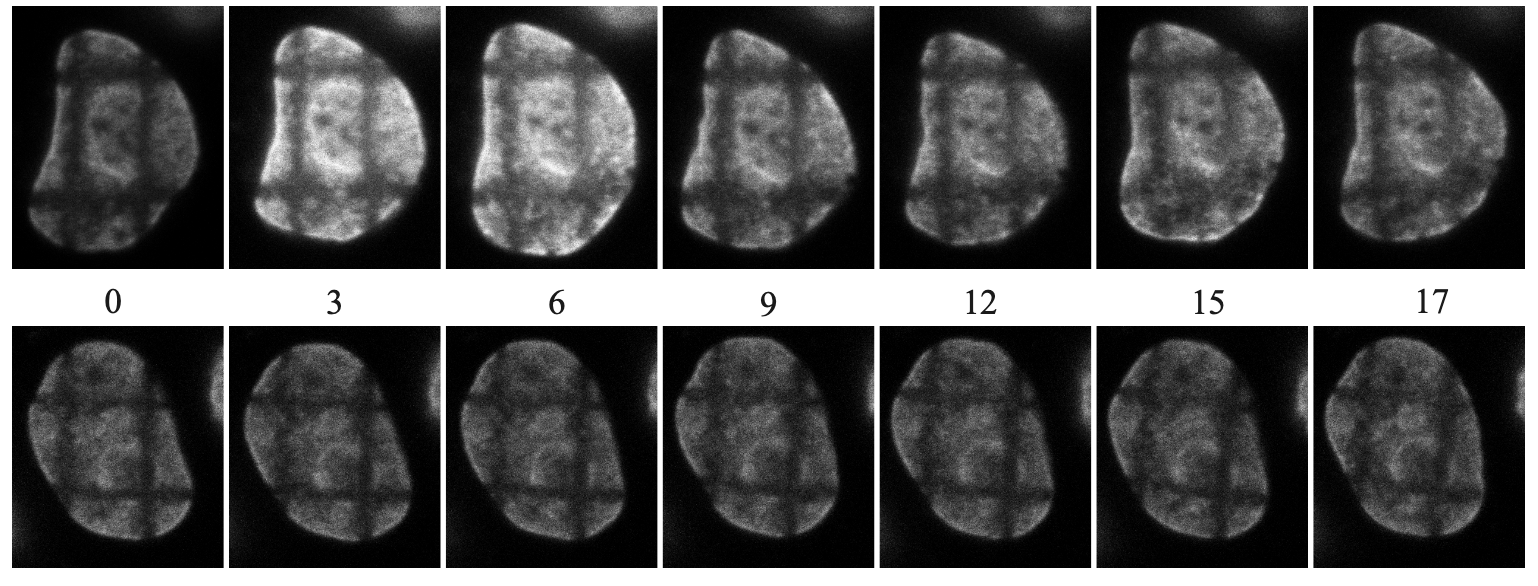
\includegraphics[width=6.5in,height=3in]{cells_img.png}}

    \caption{Примеры данных}
    \label{fig1}
\end{figure}

Процесс подготовки датасета включал следующие этапы (Рис. 8):

\begin{enumerate} 


\item \textbf{Выбор пар контуров.}
Из четырёх последовательностей формировались все возможные пары кадров (не обязательно подряд), что дало 2371 пару контуров. Все пары контуров выбираются в рамках одной последовательности, чтобы избежать трудностей с несоответствием размеров.

\item \textbf{Построение входного тензора.}
Контуры каждого кадра представляются бинарными масками $(W \times H)$. Для пары масок вычисляется тензор смещения на границе размера $(N,2)$ и формируется входной тензор размерности $(2, W, H)$, где первый и второй каналы содержат соответственно первые и вторые координаты этих векторов, записанные в точки первого контура.

\item \textbf{Генерация эталонных полей смещения.}
Ground truth поля получаются с помощью метода конечных элементов по тензору смещения на границе; выходные поля имеют размер $(W \times H)$ (Рис. 11).

\item \textbf{Нормализация интенсивности для FNO с модифицированной функцией ошибки.}
Для модели с модифицированной функцией потерь кроме бинарных масок на вход подаются также кадры интенсивностей. Предсказанное поле смещения применяется к первому кадру и сравнивается со вторым после нормализации интенсивностей. Для сравнения используется метрика $MSE$, полученная разность добаляется к функции ошибки стандартной модели.

\item \textbf{Разбиение на выборки.}
Все 2371 примеров случайным образом разделены на 70\%  для обучения, 15\% для валидации и 15\% для тестирования; батчи формируются внутри одной последовательности. 

\end{enumerate}

\begin{figure}[h]
    \centering
    {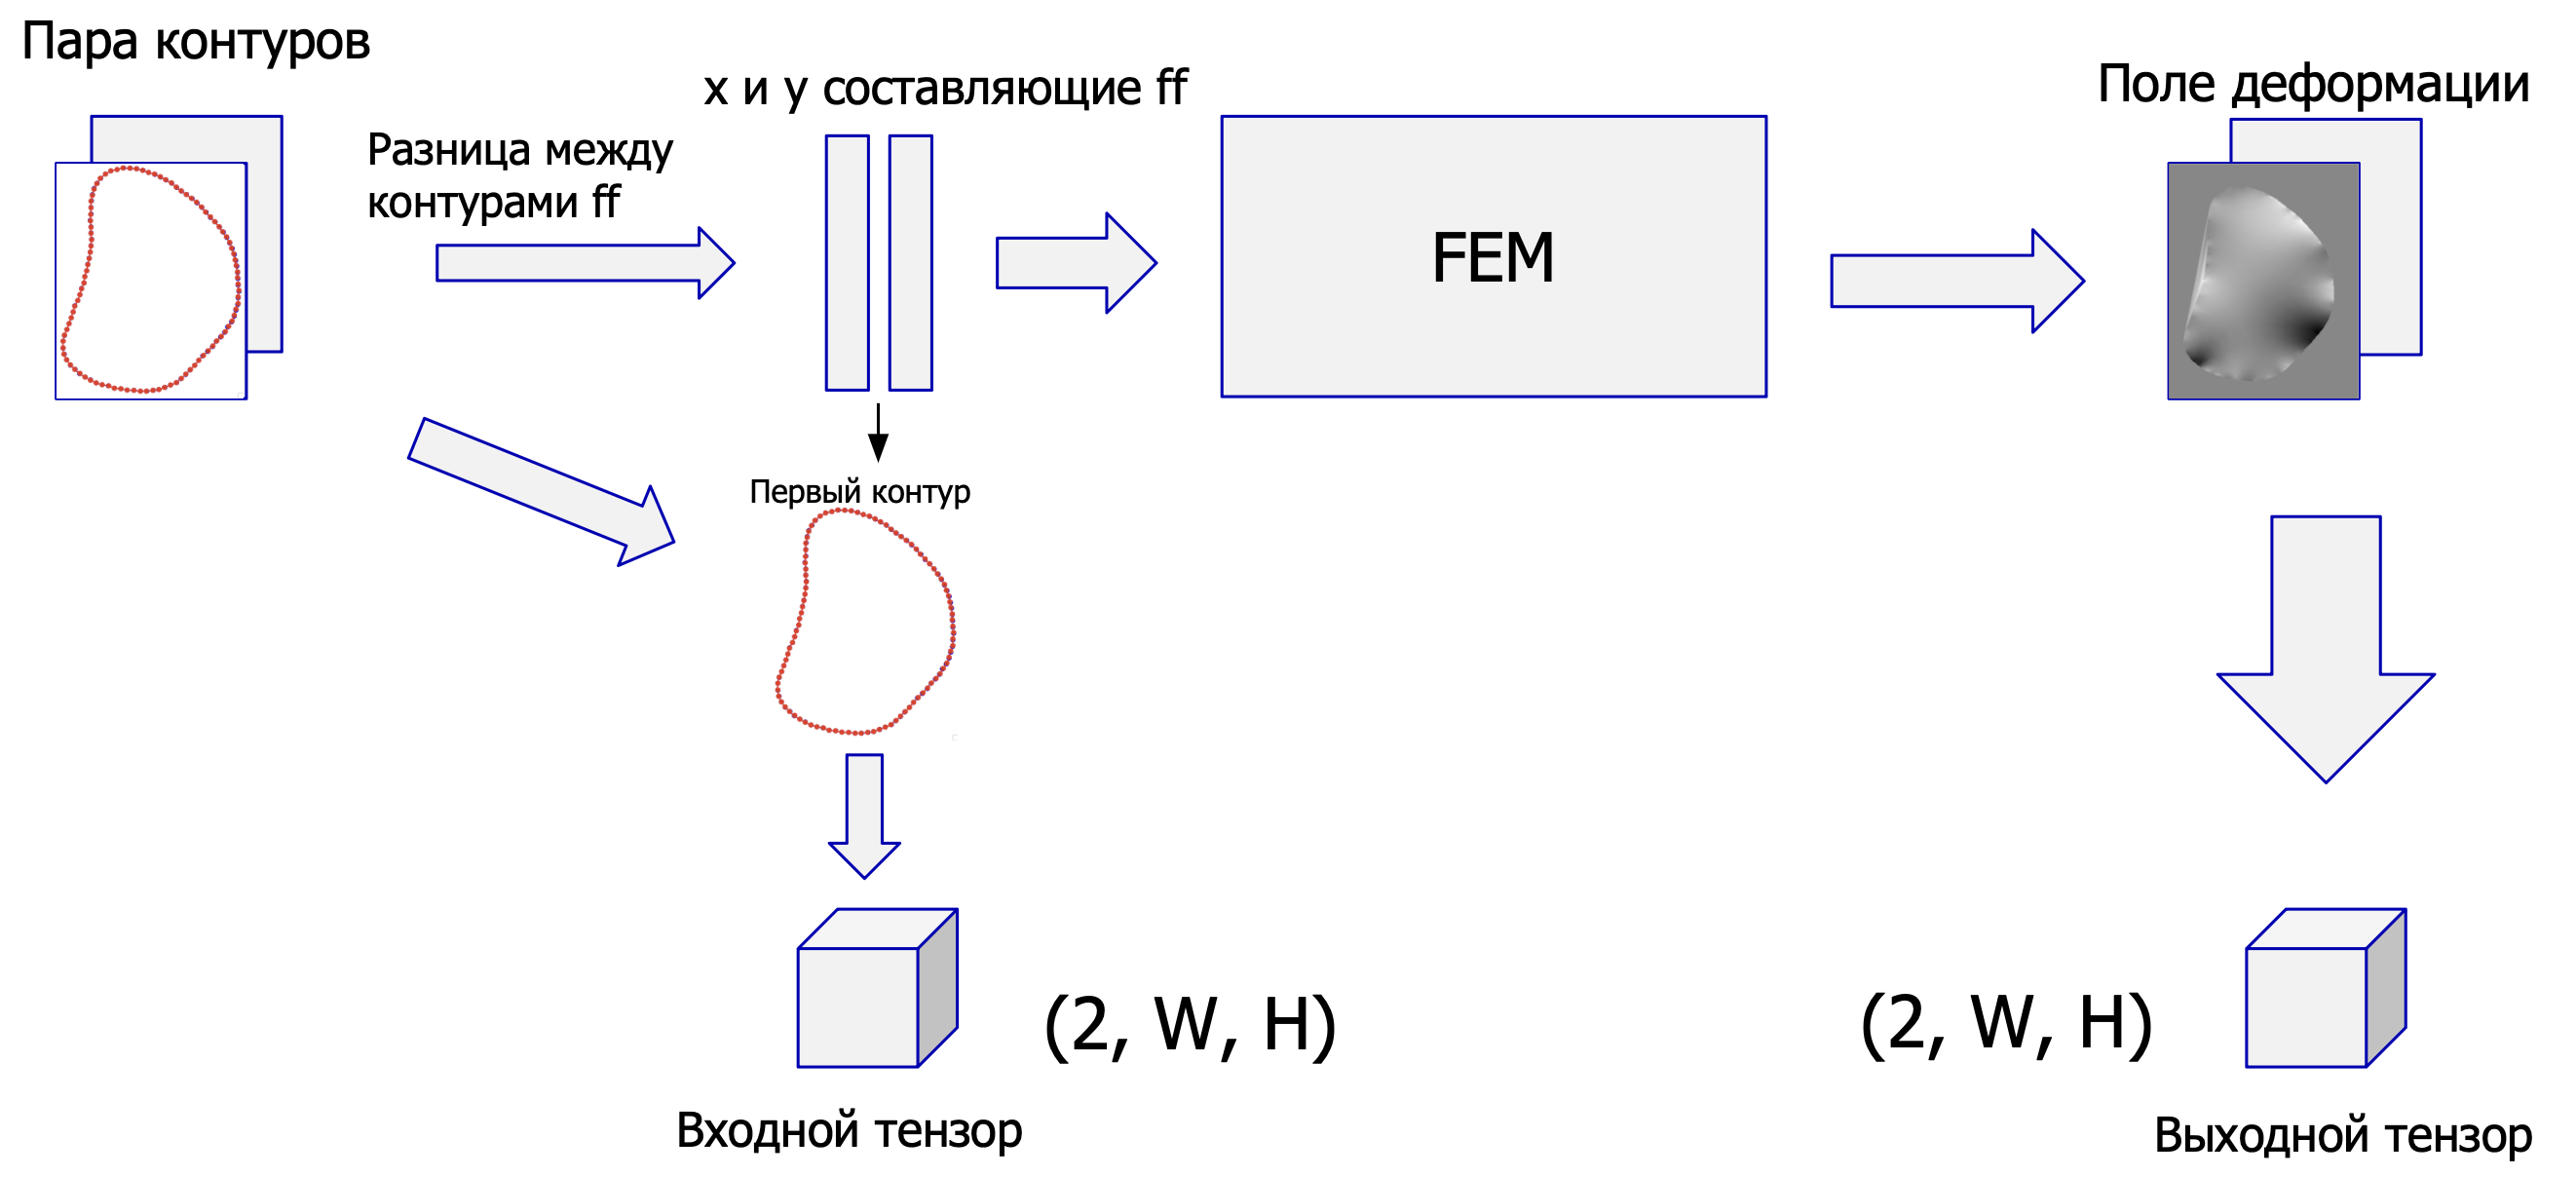
\includegraphics[width=6in,height=3in]{dataedit.png}}

    \caption{Схема подготовки данных}
    \label{fig1}
\end{figure}


В данной работе при оценке качества нежесткого совмещения используются три типа контрольных точек, все они расположены на нанесенных лазером на ядре клеток линиях сетки (Рис. 9)

\begin{itemize}
  \item \textbf{L-точки (line points)}  
    Точки, лежащие вдоль самих линий лазерной метки. Метки наносятся аргоновым лазером в виде сетки из пересекающихся линий. Для оценки ошибки совмещения вычисляется расстояние между траекторией линии в текущем и первом кадре.

  \item \textbf{I-точки (inner points)}  
    Точки пересечения клеточной сетки, лежащие внутри контура ядра. Получаются как координаты точек пересечения детектированных линий в первом кадре и используются для анализа внутренней части поля смещения.

  \item \textbf{B-точки (boundary points)}  
    Крайние точки каждого отрезка линии, располагающиеся на границе ядра. Извлекаются из результатов детекции линий как концы и служат для оценки ошибки на границе.
\end{itemize}


\begin{figure}[h]
    \centering
    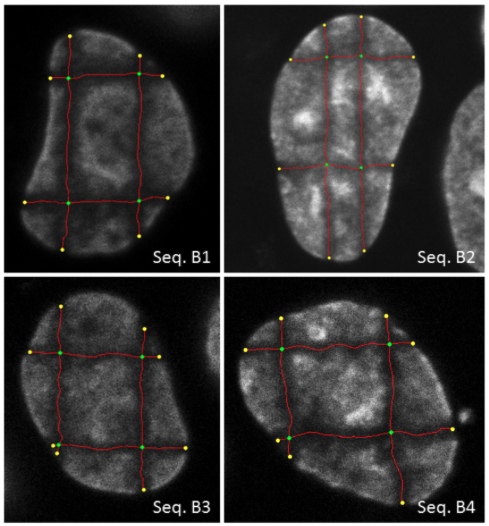
\includegraphics[width=1\linewidth]{points.png}

    \caption{Виды точек для анализа ошибок. Красным отмечены линии. Желтым - точки на границе. Зелёным - внутренние точки.}
    \label{fig1}
\end{figure}



\section{Результаты}
Чтобы оценить качество предложенного нами подхода, использовалась последовательности изображений живых клеток, полученная с помощью флуоресцентной микроскопии. Набор данных
позволил нам рассчитать результат совмещения нашего метода
и провести количественное сравнение c подходом \cite{sorokin2014nonrigid}.
Полученные в качестве результатов поля 
смещения между двумя соседними изображениями сравнимы с результатами из \cite{sorokin2014nonrigid} (Рис. 9)


% В сравнении с результатами статьи:

% \begin{figure}[h]
%     \centering
%     {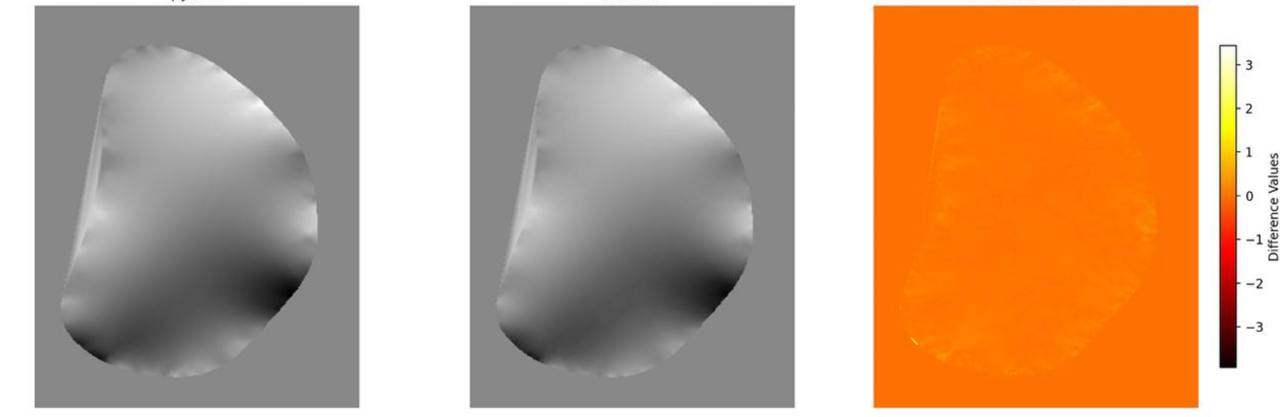
\includegraphics[width=7in,height=2.5in]{res_good_1.jpg}}\quad
%     \caption{Слева - результат алгоритма из \cite{sorokin2014nonrigid}, в центре результат реализованного метода, справа разница между результатами}
%     \label{fig1}
% \end{figure}

% Для сравнения алгоритмов был построен график ошибок (Рис. 7). По оси x отложен номер кадра, по оси y - ошибка, которая считается, как среднее расстояние между заданными точками на реальном первом изображении и полученном с помощью полей деформации алгоритма. Inner Bound и Line описывают группы точек, взятых внутри контура клеток, на границе и на определённых линиях лазерной разметки соответственно.

\begin{figure}[h]
    \centering
    {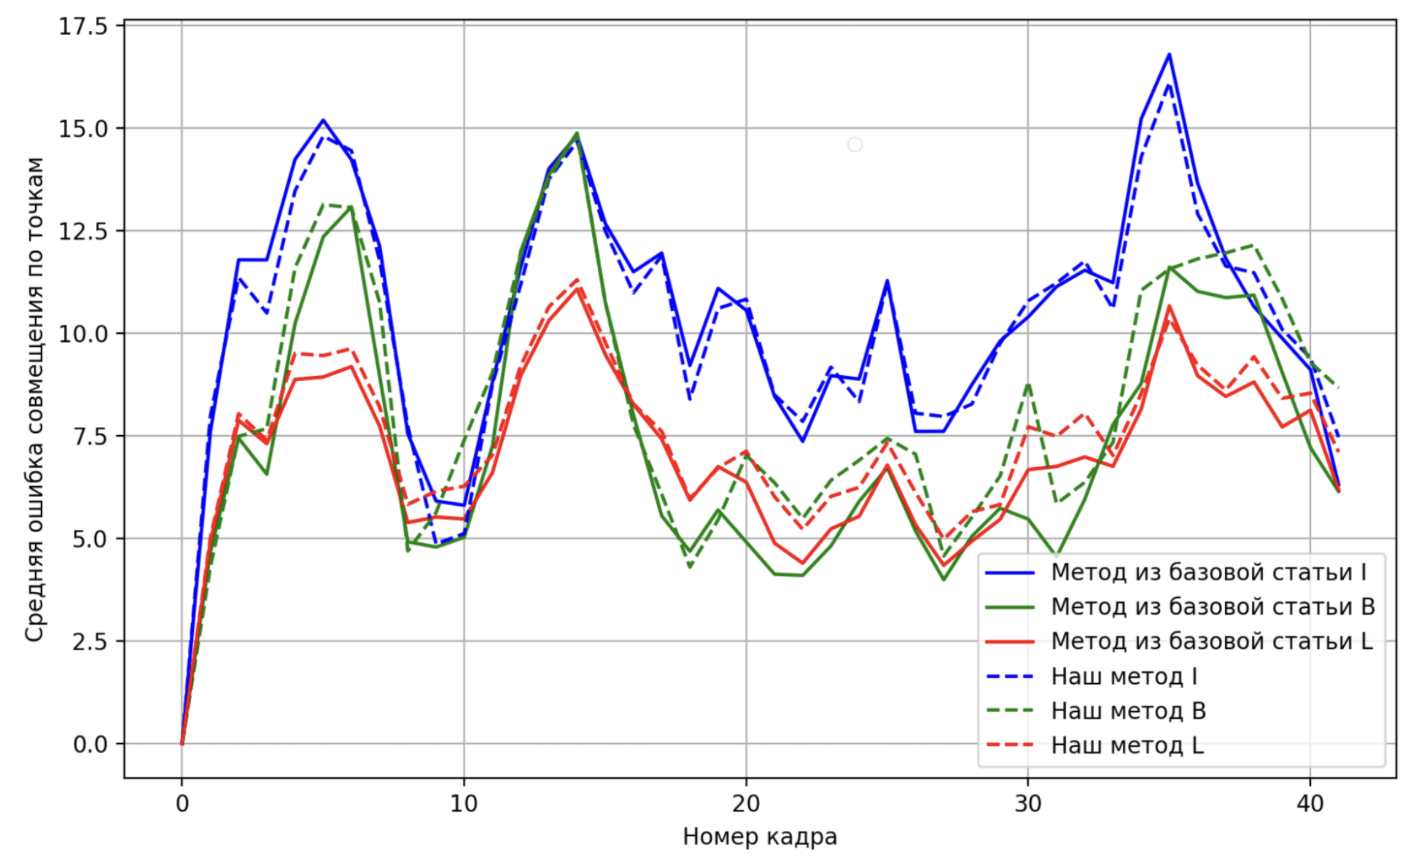
\includegraphics[width=6in,height=3.2in]{error_comp.png}}\quad
    \caption{График сравнения двух алгоритмов: метода из базовой статьи и нашей реализации}
    \label{fig1}
\end{figure}

% При обучении модели было достигнуто качество после 1000 эпох:
% \begin{itemize}
%     \item Training Loss: $0.0505$
%     \item Validation Loss: $0.1070$
%     \item Validation $R^2$: $0.9204$
% \end{itemize}


% \begin{figure}
%     \centering
%     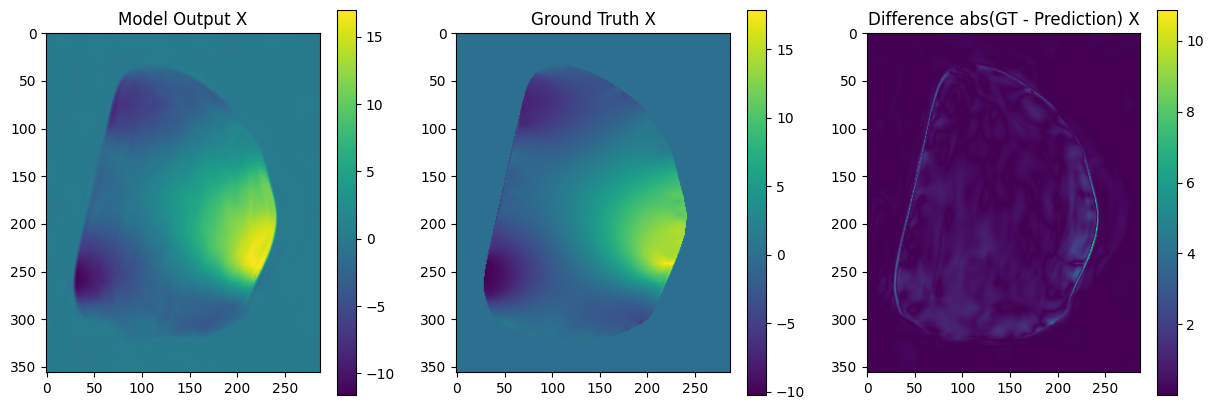
\includegraphics[width=0.75\linewidth]{11_x.jpg}
%     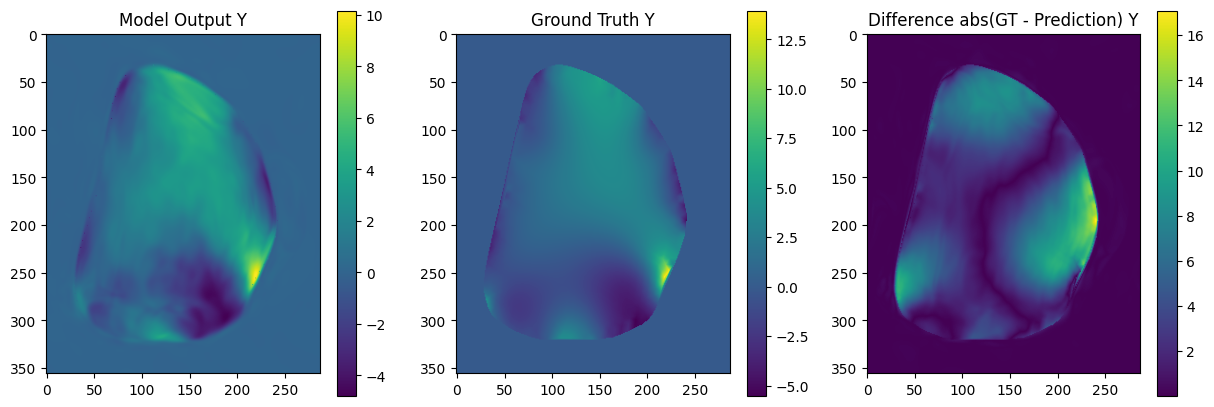
\includegraphics[width=0.75\linewidth]{11_y.png}
%     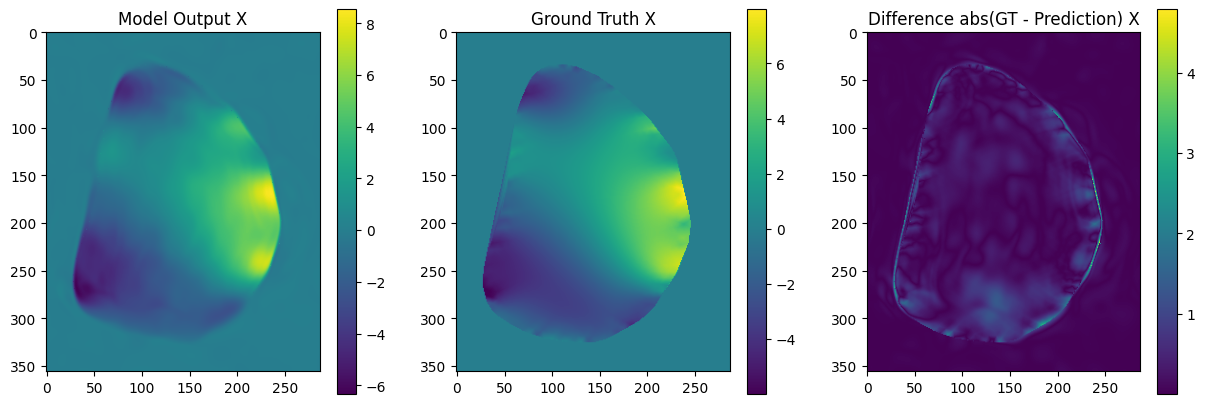
\includegraphics[width=0.75\linewidth]{17_x.png}
%     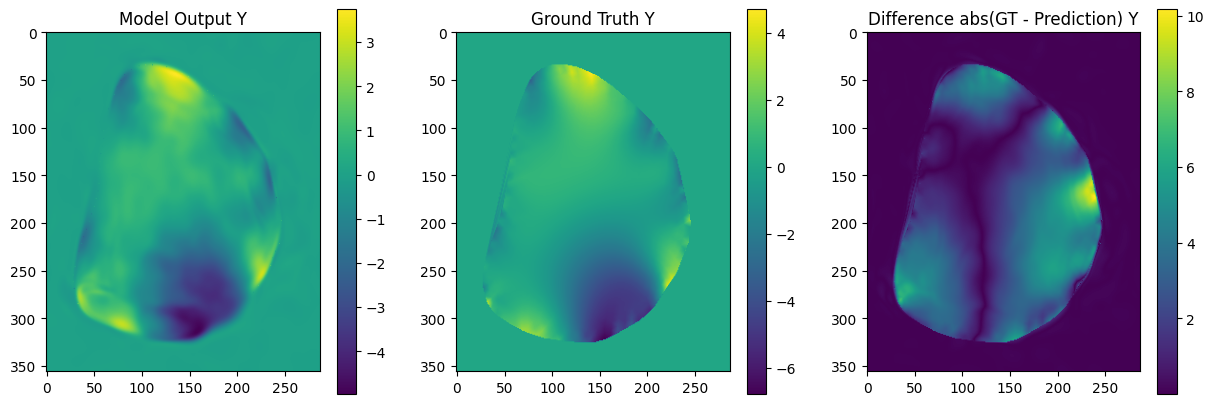
\includegraphics[width=0.75\linewidth]{17_y.png}
%     \caption{Примеры работы модели}
%     \label{fig:enter-label}
% \end{figur



\begin{figure}[h]
  \centering
  % Верхний график
  \begin{subfigure}[b]{0.7\textwidth}
    \centering
    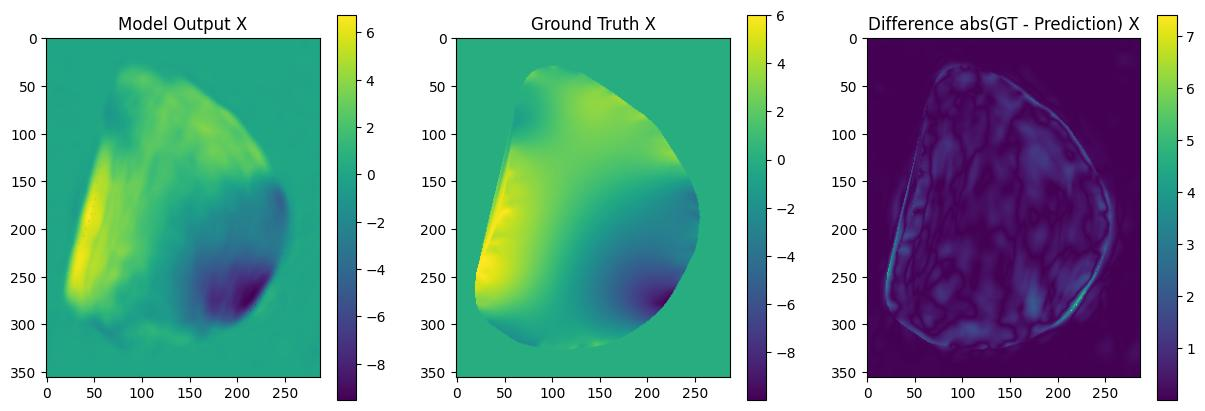
\includegraphics[width=\linewidth]{model_field_2.jpg}
    \label{fig:mf1}
  \end{subfigure}

  \vspace{1em}

  % Нижний график
  \begin{subfigure}[b]{0.7\textwidth}
    \centering
    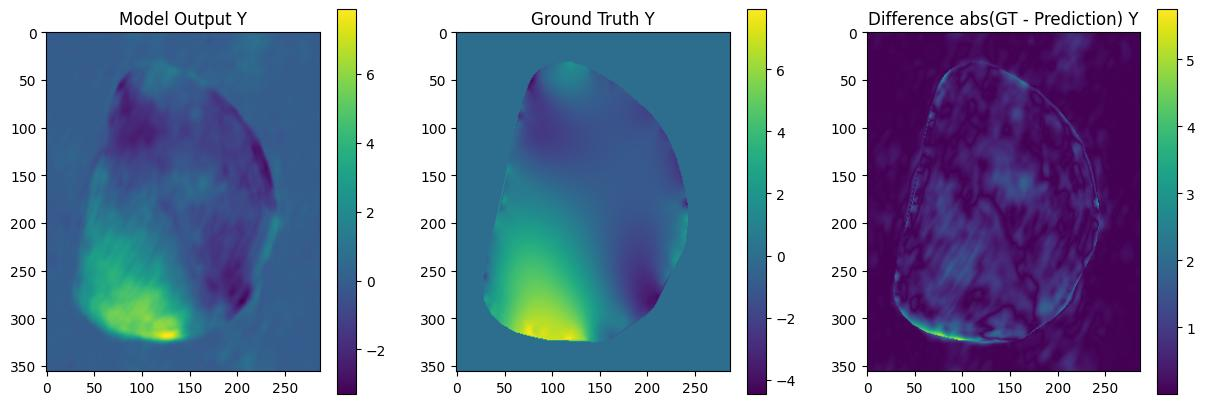
\includegraphics[width=\linewidth]{model_field_1.jpg}
    % \caption{Поле деформации модели 2}
    \label{fig:mf2}
  \end{subfigure}

  \caption{Пример выхода модели в сравнении с ground truth значением}
  \label{fig:field_models}
\end{figure}

\paragraph{Вычисление ошибки совмещения.}  
В соответствии с \cite{sorokin2014nonrigid}, ошибка совмещения \(\bar{e}\) определяется как усреднённое по всем временным точкам и всем точечным признакам евклидово расстояние между позициями, полученными после совмещения, и вручную аннотированными эталонными позициями:
\[
\bar{e} = \frac{1}{N_{\rm frames} \cdot N_{\rm features}}
\sum_{t=1}^{N_{\rm frames}}
\sum_{k=1}^{N_{\rm features}}
\bigl\|\,\mathbf{x}_{t,k}^{\rm reg} - \mathbf{x}_{t,k}^{\rm ref}\bigr\|_2,
\]
где \(N_{\rm frames}\) — число кадров, \(N_{\rm features}\) — число line features в каждом кадре, \(\mathbf{x}_{t,k}^{\rm reg}\) и \(\mathbf{x}_{t,k}^{\rm ref}\) — зарегистрированная и эталонная позиции \(k\)-й точки в кадре \(t\).

Для сравнения алгоритмов был построен график ошибок (Рис. 10, 12). По оси x отложен номер кадра, по оси y - ошибка, которая считается, как среднее расстояние между заданными точками на реальном первом изображении и полученном с помощью полей смещения алгоритма. I, B и L описывают группы точек, взятых внутри контура клеток, на границе и на определённых линиях лазерной разметки соответственно (Таблица 2).

\begin{landscape}
\begin{table}[ht]
    \centering
    \resizebox{\textwidth}{%
      \begin{tabular}{|l|S|S|S|S|S|S|S|S|S|S|S|S|S|S|S|S|S|}
        \hline
        & \textbf{Парам.}
        & \multicolumn{3}{c|}{\textbf{Посл. B1}}
        & \multicolumn{3}{c|}{\textbf{Посл. B2}}
        & \multicolumn{3}{c|}{\textbf{Посл. B3}}
        & \multicolumn{3}{c|}{\textbf{Посл. B4}}
        & \multicolumn{3}{c|}{\textbf{Среднее}}
        & \textbf{Среднее} \\
        \hline
        \textbf{Модель / Тип ошибки}
        & 
        & {I} & {B} & {L}
        & {I} & {B} & {L}
        & {I} & {B} & {L}
        & {I} & {B} & {L}
        & {I} & {B} & {L}
        & {} \\
        \hline
        FEM                     & –    & 10.37 &  8.34 &  7.46 &  5.87 &  3.86 &  3.69 &  3.28 &  3.83 &  3.14 &  3.54 &  2.46 &  2.84 &  5.77 & 4.62 & 4.28 & 4.89 \\
        FNO (small)            & 1.5M & 10.86 &  9.55 &  8.66 &  6.38 & \textbf{3.81} &  3.96 & \textbf{3.05} & \textbf{3.30} & \textbf{2.99} & \textbf{3.53} &  2.59 &  2.94 & 5.96 & 4.81 & 4.64 & 5.14 \\
        FNO (large)            & 4M   & 12.65 &  9.94 & 10.25 & \textbf{5.67} & \textbf{3.61} &  3.80 &  3.32 & \textbf{3.13} &  3.17 & \textbf{3.25} &  2.87 & \textbf{2.82} & 6.22 & 4.89 & 5.01 & 5.37 \\
        FNO + intensity loss (small) & 1.5M & \textbf{10.29} &  9.01 &  7.66 &  6.27 & \textbf{3.64} &  3.83 &  3.65 & \textbf{3.38} &  3.33 &  3.90 & \textbf{2.40} &  2.91 & 6.03 & \textbf{4.61} & 4.43 & 5.02 \\
        FNO + intensity loss (large) & 6M   & 10.85 &  8.90 &  8.04 & \textbf{5.72} & \textbf{3.52} & \textbf{3.66} & \textbf{3.26} & \textbf{3.73} &  3.16 &  3.91 &  2.52 &  2.90 & 5.94 & 4.67 & 4.44 & 5.01 \\
        UNO                    & 14M  & \textbf{9.10}  &  9.11 & \textbf{7.36} &  6.05 & \textbf{3.81} &  3.88 & \textbf{3.22} & \textbf{3.81} &  3.30 & \textbf{3.51} & \textbf{2.41} &  3.00 & \textbf{5.47} & 4.79 & 4.39 & \textbf{4.87} \\
        \hline
      \end{tabular}%
    }
    \vspace{}
    \caption{Результаты работы различных моделей на четырёх последовательностях. 
    L — ошибка совмещения точек на линиях. 
    I — ошибка совмещения внутренних точек. 
    B — ошибка совмещения точек на границе. Жирным выделены те результаты, которые превзошли метод FEM}
    \label{tab:fno-results}
\end{table}
\end{landscape}
\paragraph{Сравнение моделей.}  
\begin{itemize}
  \item UNO продемонстрировала наибольшее снижение \(\bar{e}\) в среднем по всем последовательностям, благодаря сочетанию локального и глобального захвата признаков.
  \item FNO с изменённой функцией потерь (large) опередила FEM на последовательностях B2 и B3  по всем метрикам, что подтверждает пользу учёта реконструированного интенсивностного кадра в функции потерь.
  \item Увеличение числа параметров (\textit{large} vs \textit{small}) для FNO снизило ошибку I.
\end{itemize}

\begin{figure}[h]
  \centering
  %--- верхний ряд
  \begin{subfigure}[t]{0.5\textwidth}
    \centering
    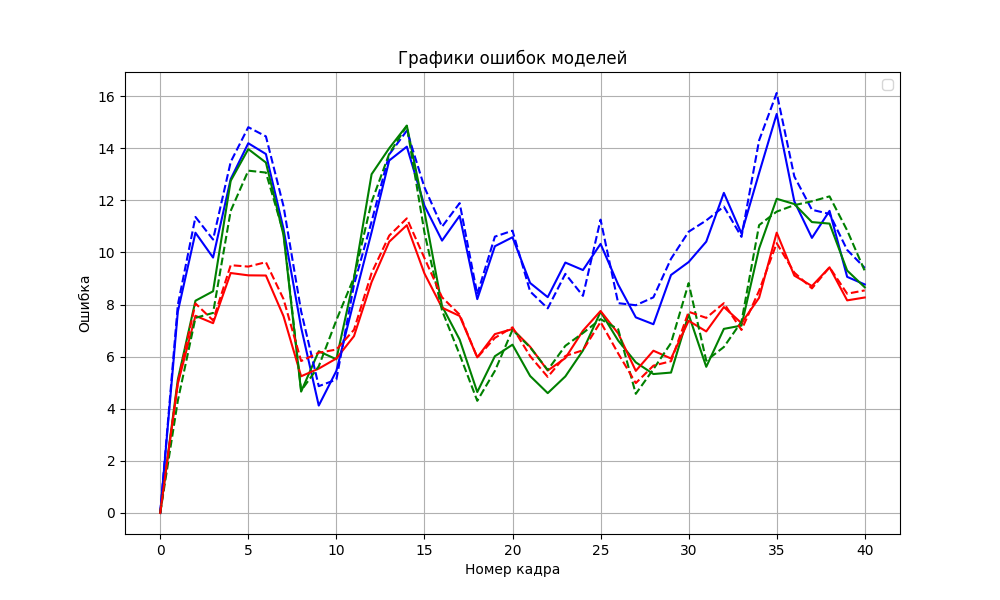
\includegraphics[width=\linewidth]{error_plot_model_Series015.png}
    \caption{Ошибки U-NO на последовательности B1}
    \label{fig:mg1}
  \end{subfigure}\hfill
  \begin{subfigure}[t]{0.5\textwidth}
    \centering
    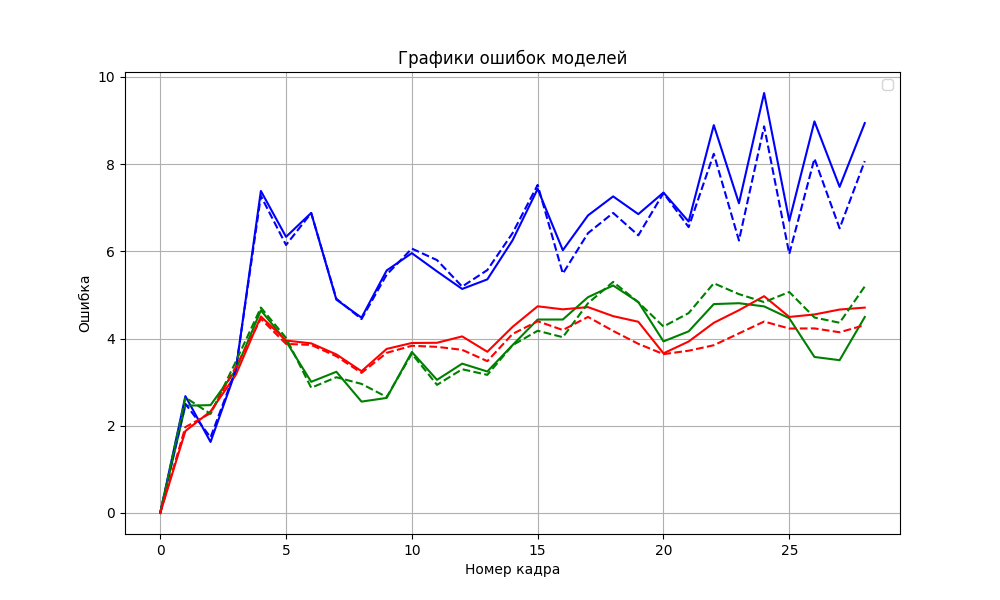
\includegraphics[width=\linewidth]{error_plot_model_Series020-021.png}
    \caption{Ошибки U-NO на последовательности B2}
    \label{fig:mg2}
  \end{subfigure}

  \vspace{1em}

  %--- нижний ряд
  \begin{subfigure}[t]{0.5\textwidth}
    \centering
    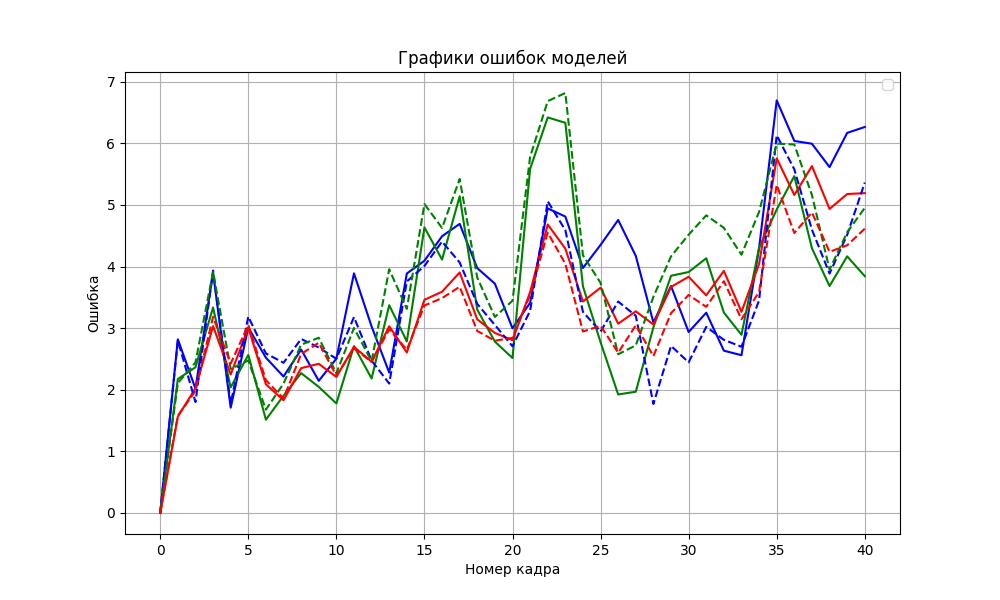
\includegraphics[width=\linewidth]{error_plot_model_Series036.png}
    \caption{Ошибки U-NO на полсдовательности B3}
    \label{fig:mg3}
  \end{subfigure}\hfill
  \begin{subfigure}[t]{0.5\textwidth}
    \centering
    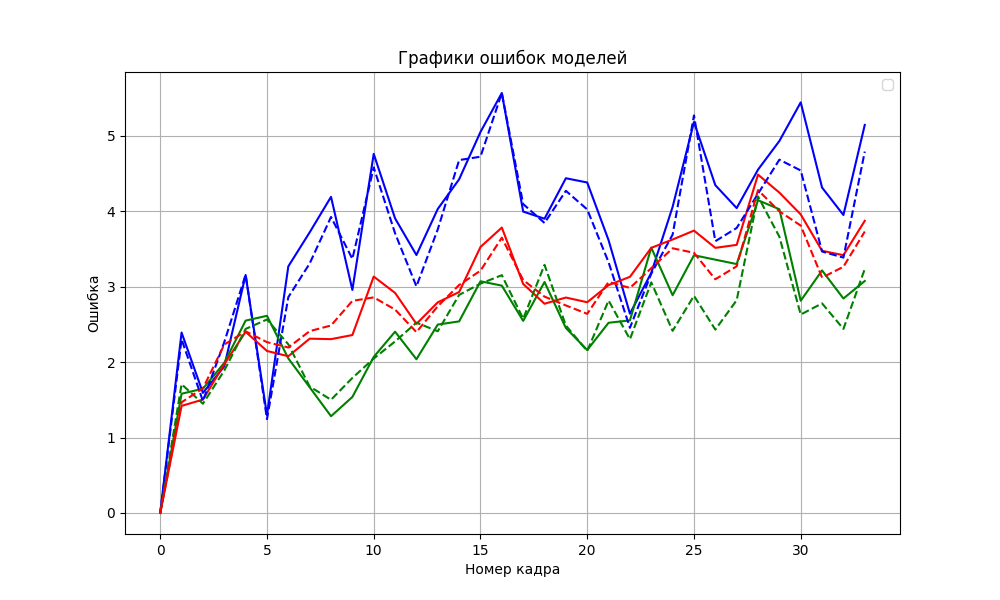
\includegraphics[width=\linewidth]{error_plot_model_Series060.png}
    \caption{Ошибки U-NO на полсдовательности B4}
    \label{fig:mg4}
  \end{subfigure}

  \caption{Сравнение ошибок U-NO и FEM на всех последовательностях. Красным отмечены ошибки типа L, зеленым ошибки типа B, синим ошибки типа I. Пунктиром отмечены ошибки МКЭ, сплошной линией ошибки модели.}
  \label{fig:all_model_graphs}
\end{figure}

На графиках (Рис. 13) хорошо видно, что модель UNO работает лучше, чем другие модели, так как соответствующая U-NO кривая лежит ниже, чем линии остальных моделей для всех видов тчек.

\begin{figure}[ht]
  \centering
  %--- верхний ряд
  \begin{subfigure}[t]{0.5\textwidth}
    \centering
    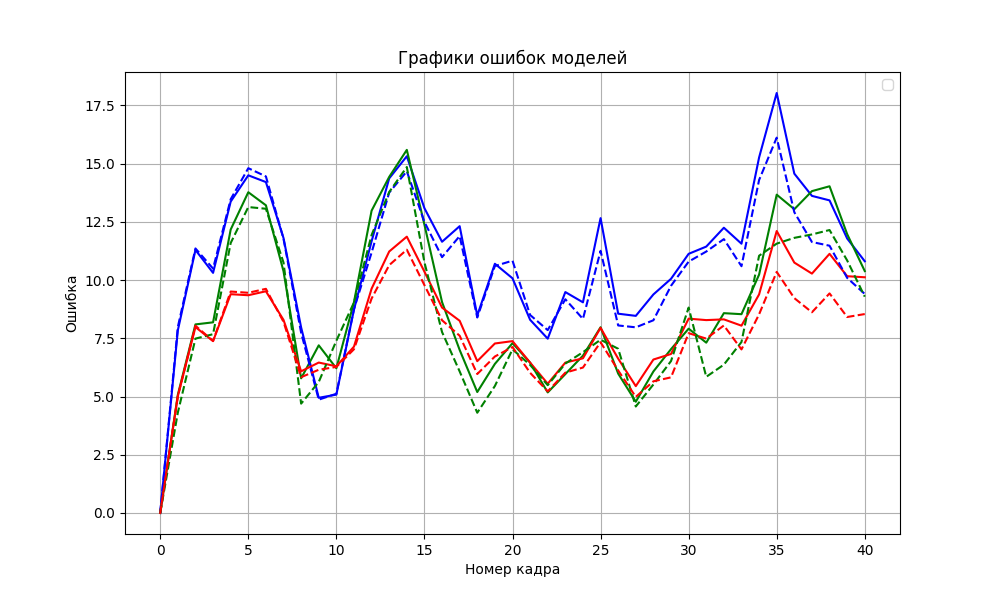
\includegraphics[width=\linewidth]{norm.png}
    \caption{Ошибки FNO + изменённая функция потерь (small) на последовательности B1}
    \label{fig:mg1}
  \end{subfigure}\hfill
  \begin{subfigure}[t]{0.5\textwidth}
    \centering
    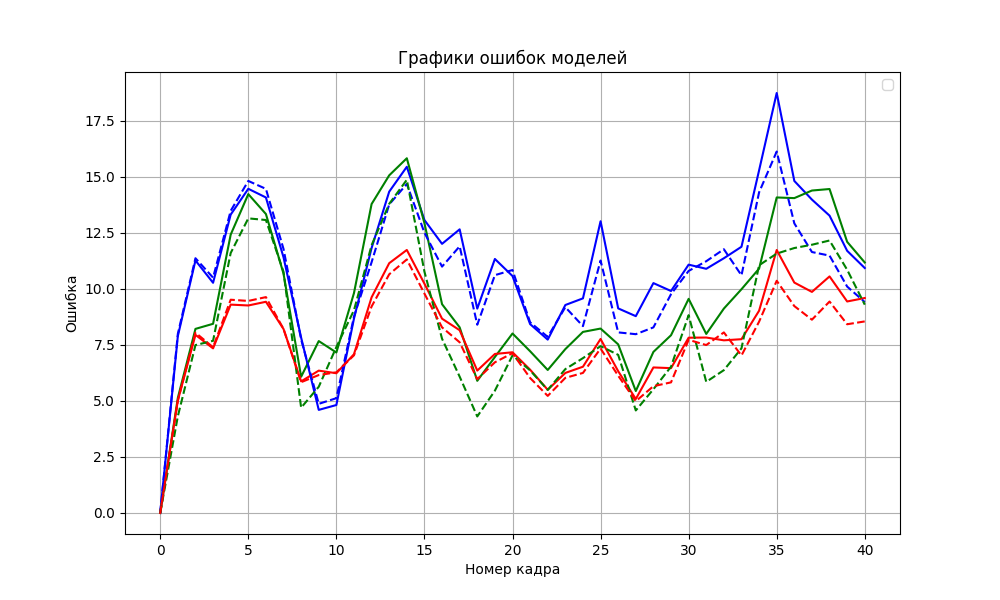
\includegraphics[width=\linewidth]{norm_2.png}
    \caption{Ошибки FNO large на последовательности B1}
    \label{fig:mg2}
  \end{subfigure}

  \vspace{1em}

  %--- нижний ряд
  \begin{subfigure}[t]{0.5\textwidth}
    \centering
    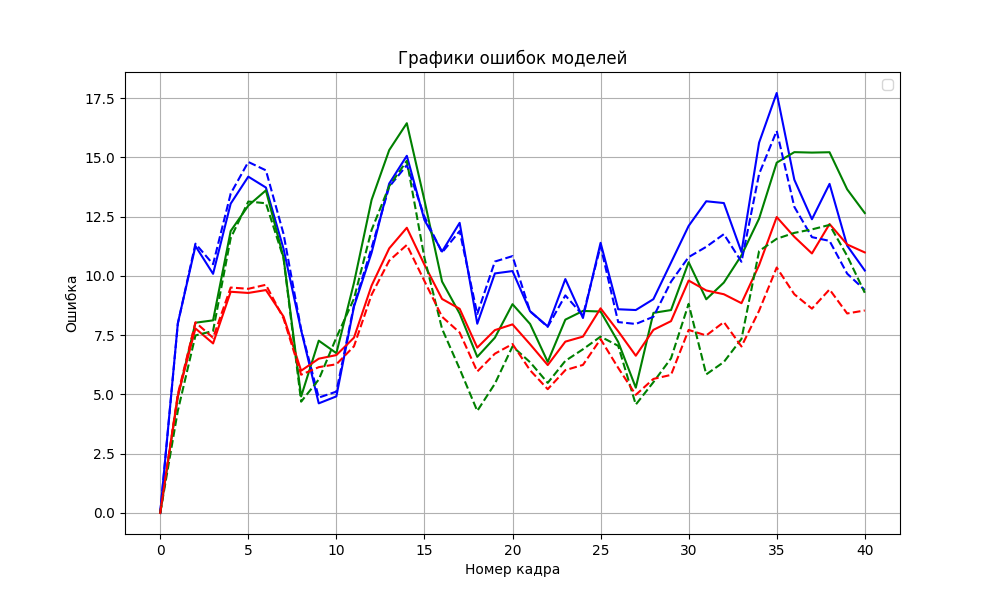
\includegraphics[width=\linewidth]{bad.png}
    \caption{Ошибки FNO + изменённая функция потерь (large) на последовательности B1}
    \label{fig:mg3}
  \end{subfigure}\hfill
  \begin{subfigure}[t]{0.5\textwidth}
    \centering
    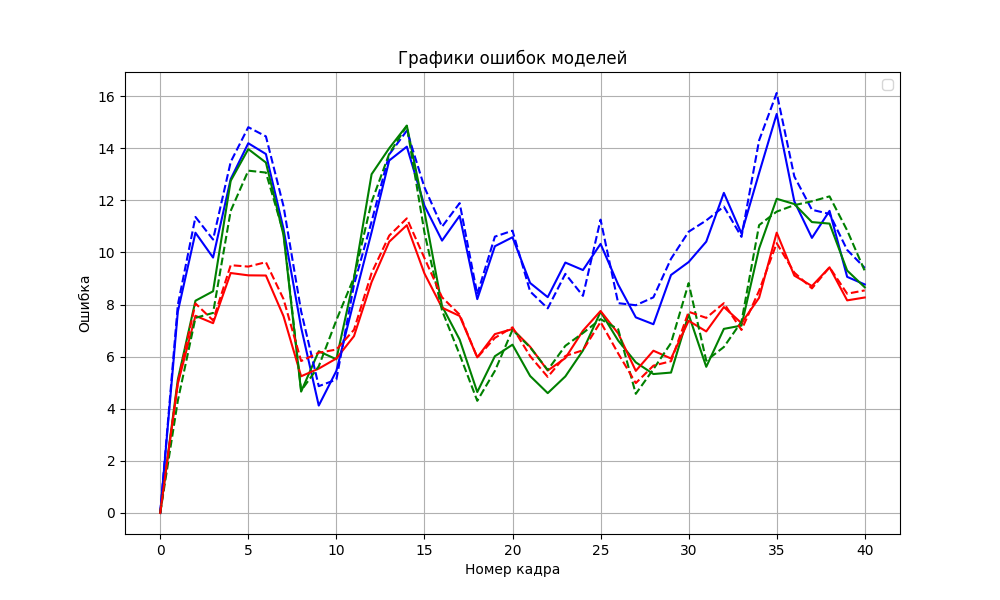
\includegraphics[width=\linewidth]{best.png}
    \caption{Ошибки U-NO на последовательности B1}
    \label{fig:mg4}
  \end{subfigure}

  \caption{Сравнение ошибок разных моделей на последовательности B1. Красным отмечены ошибки типа L, зеленым ошибки типа B, синим ошибки типа I. Пунктиром отмечены ошибки МКЭ, сплошной линией ошибки модели.}
  \label{fig:all_model_graphs}
\end{figure}










\section{Заключение}

В ходе работы была реализована классическая схема нежёсткого совмещения изображений клеточных ядер на базе численного решения уравнения Навье методом конечных элементов, описанного в базовой статье \cite{sorokin2014nonrigid}. Данный подход продемонстрировал приемлемую точность регистрации.

Был предложен гибридный метод нежесткого совмещения, в котором традиционный подход с конечными элементами сочетается с обучаемыми операторами в спектральном пространстве — нейронным оператором Фурье.

Проведённый численный анализ на четырх последовательностях показал, что среди всех рассмотренных вариантов наилучшие результаты по среднему значению ошибки продемонстрировала модель U-shaped Neural Operator (UNO). Это подтверждает, что интеграция U-образной структуры эффективно улавливает детали деформации.

Все описанные методы (МКЭ, FNO, U-NO и модифицированный FNO с новой функцией потерь) программно реализованы на языке Python 3. Реализация включает модуль загрузки и предобработки кадров, архитектуры нейронных операторов на PyTorch, а также скрипты для обучения, валидации и визуализации результатов, что обеспечивает воспроизводимость и удобство дальнейшего развития алгоритмов в рамках научных и прикладных задач.





\bibliography{refs} % Entries are in the refs.bib file



\end{document}
